\chapter{Aplicación}
\label{ch:aplicación}


% El siguiente es el texto que aparece en el encabezamiento del proyecto fin de grado (si se quiere que sea distinto al nombre del capítulo))
%\chaptermark{PFG}
Dentro de este capitulo se pueden encontrar los apartados referentes al analisis y diseño de la aplicacion Baldugenda y el desarrollo y pruebas seguido durante el proyecto.

\section{Análisis y diseño}
\label{secc:análisis y diseño}
Se han dividido el apartado de análisis y diseño en 5 apartados donde se podrá encontrar la arquitectura usada y un pequeño análisis de alternativas vistas, después estarán los casos de uso de la versión del último ciclo de Baldugenda. También habrá una sección donde se detalla el modelo de datos usado, para posteriormente hablar sobre las interfaces de usuario y para terminar en un análisis de diseño. 
\subsection{Arquitectura}
\label{subsecc:arquitectura}

Para ver cómo funciona la aplicación, tenemos que entender primero su arquitectura. Baldugenda tiene una arquitectura \acrshort{mvc}, esto quiere decir que tiene separadas las partes de los datos, la lógica de negocio y la interfaz de usuario.
El modelo vista controlador, es un patrón de arquitectura de software que separa los datos y la lógica de negocio. Este tipo de arquitectura es muy útil si se va a trabajar en un dispositivo móvil, ya que actualmente los datos se quieren usar para Android pero puede que en un futuro se quisieran usar en una aplicación web, la migración sería sencilla. Esto es gracias a la distribución que ofrece Android con el uso de los layouts y de sus \glspl{activity}.
El funcionamiento que ofrece Android por medio de sus actividades funciona como controlador en la arquitectura MVC siendo la vista los layouts.

\begin{figure}[H] 
  \begin{center} 
    \scalebox{0.4}{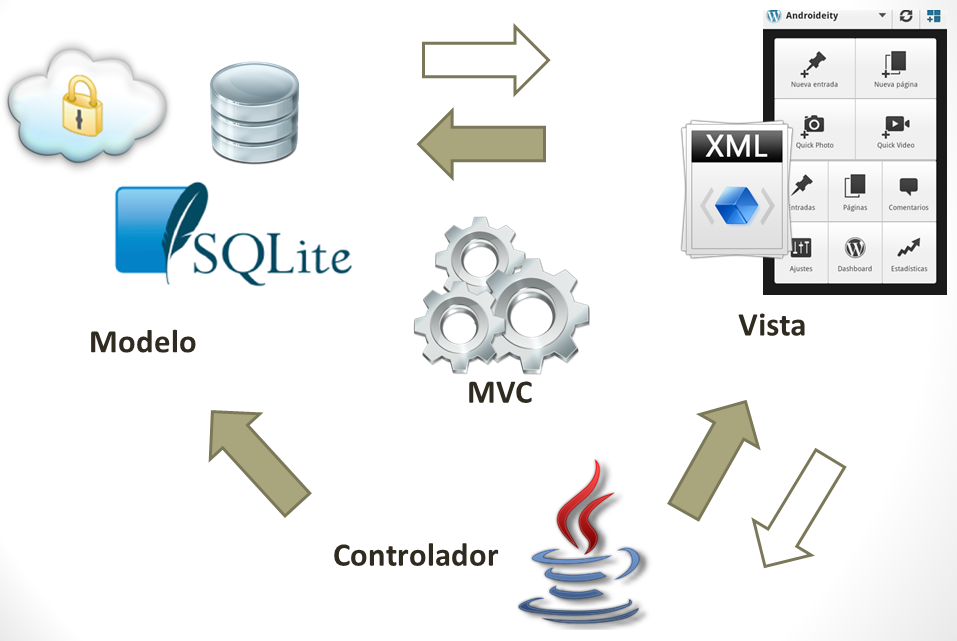
\includegraphics{figs/modeloMVC.png}} 
    \caption{Modelo MVC de Androideity.com} 
    \label{fig:ModeloMVC} 
  \end{center} 
\end{figure}

\subsubsection{Arquitecturas identificadas}
\label{subsubsecc:Arquitecturas identificadas}

Se tuvieron en cuenta diferentes alternativas a la hora de desarrollar la arquitectura. En este apartado, se explicarán las alternativas y la arquitectura definitiva usada en el proyecto.

\myparagraph{Alternativa: Nativa}

El desarrollo de una aplicación nativa ofrece el acceso a la gran mayoría de los recursos de los que dispone el dispositivo móvil.
Se puede acceder a todos sus componentes sin necesidad de plugins o software de terceros.
La desventaja es que solo funcionaria con dispositivos del sistema operativo para el que se está desarrollando.

\myparagraph{Alternativa: Aplicación Web}

El desarrollo de una aplicación web conseguiría que todos los dispositivos móviles con acceso a internet pudieran acceder a la aplicación.
Una de las desventajas es el acceso a la información propia del dispositivo, como puede ser la cámara o el estado de la conexión.
\myparagraph{Alternativa: Web-app nativo}

Para esta alternativa, se podría usar software especializado en el desarrollo, como puede ser Cordova\cite{Cordova} o Phonegap\cite{Phonegap}. Este software nos serviría para desarrollar una app en formato web y convertirla en formato nativo.
El problema surgiría al querer acceder a los recursos, debido a que tendríamos que depender de librerías de terceros para realizar las consultas.
\myparagraph{Arquitectura definitiva:}

En Baldugenda se optó por la alternativa nativa, puesto que el desarrollo de una aplicación Android era uno de los propósitos de este proyecto, por la agilidad que se tendría a la hora de desarrollar y por haber realizado cursos  y proyectos anteriormente con aplicaciones nativas.
El uso de esta arquitectura viene asociado al modelo MVC, que se ha mencionado anteriormente.  La ventaja de usar este modelo es que las posibilidades de migrar el código a otro tipo de arquitectura son altas, y con coste más reducido, que tener que implementarla desde cero.
Para esta aplicación, se separó el modelo de datos de la parte de la lógica del negocio para que si en un futuro se quisiera implementar en otro sistema operativo, como puede ser IOS, sólo se tendría que realizar la conversión del controlador y el trabajo se podría dividir a distintas personas.

\subsubsection{Formato de guardado}
\label{subsubsecc:formato de guardado}

Aparte del tipo de aplicación que se tenía que realizar, se tuvo en cuenta el formato que se usaría en la aplicación para guardar los datos.
Se decidió usar de base de datos Sqlite, ya que se había trabajado con anterioridad con este tipo de base de datos en las anteriores aplicaciones en Android que se habían realizado, y el manejo era sencillo, cómodo y no pesaba en exceso al guardarlo en el dispositivo móvil.
Para la gestión de las opciones del programa, se optó por el formato de XML. En estos ficheros se guarda la información de configuración de la aplicación, como puede ser la cuenta de Gmail predeterminada, para evitar pedirla cada vez que se abre la app.
Al trabajar con los servicios de Google, se ha tenido que usar JSON para recibir la información de la API de Google Calendar, y después leer esa información y pasarla a la base de datos.
Para trabajar con los ficheros de Sqlite se decidió usar un software llamado Sqliteman.
Este software nos da acceso a la base de datos, nos permite modificarla y comprobar la forma que tiene, ya que al crear la base de datos y las tablas por medio de Android, las consultas puede fallar y no funcionar como se esperaba.

\subsection{Casos de uso}
\label{subsecc:casos de uso}

En el apartado de Modelo de datos ya se ha hablado de las clases sobre las que gira la aplicación.
En este apartado, se detallarán los casos de uso. Al haber 3 clases principales, se separaran los casos de uso en 4  tipos, por un lado, los casos de uso propios de cada clase y por otro, un grupo general para los casos de uso que afectan a la mayoría.
Los nombres de los casos de uso son auto explicativos, así que la mayoría de los casos no se explicaran a conciencia.

\subsubsection{Casos de uso sobre Asignatura}
\label{subsubsecc:Casos de uso sobre Asignatura}

Para empezar, se explicará el caso de uso \textbf{Crear asignatura}, este caso de uso da la posibilidad al usuario de crear una asignatura. Este tipo de objeto será el que tenga más peso ya que sin una asignatura no se podrá realizar nada en la aplicación.
Cuando el usuario le dé a crear asignatura, se le pedirá que ingrese los campos como nombre, escoja el tipo de evaluación, y la nota que tiene esa asignatura.
También hay una opción de añadir enlaces donde se irán generando campos de texto para que el usuario escriba los enlaces interesantes para esa asignatura, como por ejemplo podría ser la web de la asignatura o directamente alguna web que el profesor haya dicho que estará relacionada directamente. Si éstos son enlaces  enlaces a páginas web, los usuarios tendrán la posibilidad de mediante un click acceder a ellos en el caso de uso de visualizar asignatura.
Al usuario se le mostrará un texto diciéndole que la asignatura se ha creado con éxito.

Otro caso de uso sería el de \textbf{Modificar asignatura}, el usuario podrá escoger una asignatura por medio de la lista, o estando ya dentro de una asignatura darle a modificar. De esa forma, el usuario pasará a otra ventana donde se le mostrará los datos editables de esa asignatura.
El usuario podrá modificar todo excepto el nombre, los demás campos cogerán el valor que tiene la asignatura guardada, y permitirá modificarlos aunque los  cambios no se guardarán hasta que el usuario pulse el botón de guardar.
En ese momento, la asignatura se modificará en la base de datos y al usuario se le mostrarán por un lado de nuevo la asignatura con los datos guardados y por otro, un mensaje mostrando que su asignatura se ha modificado con éxito.


Aparte de Modificar asignatura se puede \textbf{Borrar asignatura}, con esta opción el usuario hará lo mismo que en el caso de modificar asignatura, pero en vez de mostrarle la nueva ventana con los datos de la asignatura, ahora se le mostrará un mensaje de si está seguro que desea borrarla.
Al decir que sí el usuario, la asignatura se borrará o devolverá un mensaje de error informando el motivo por el que no se ha podido borrar.
Sólo se permite borrar asignatura que no tengan exámenes dentro, esto se decidió así ya que si no, supondría un borrado en cascada, y el coste que produciría eso sería muy elevado ya que también se tendrían que borrar los eventos en el calendario de Google de todos los exámenes de esa asignatura.


\begin{figure}[H]
 \centering
  \subfloat[Borrado en Asignatura]{
   \label{f:Borrado en Asignatura}
    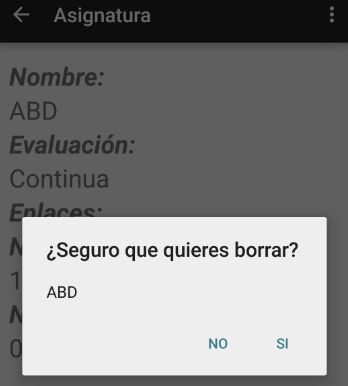
\includegraphics[width=0.4\textwidth]{figs/BorradoAsignatura.png}}
  \subfloat[Borrado en Lista Asignaturas]{
   \label{f:Borrado en Lista Asignaturas}
    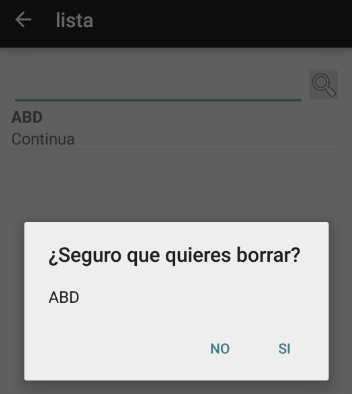
\includegraphics[width=0.4\textwidth]{figs/BorradoListaAsignaturas.png}}
 \caption{Tipos de borrado asignatura}
 \label{f:Tipos de borrado asignatura}
\end{figure}

Para que el usuario pueda visualizar todas las asignaturas está el caso de uso \textbf{Ver lista asignaturas}, en esta ventana se pueden visualizar las asignaturas en forma de lista y en cada recuadro se mostrará el nombre de la asignatura y el tipo de evaluación que tiene seleccionada.
Desde esta actividad se puede acceder a todas las actividades referentes a una asignatura. Se puede modificar y borrar una asignatura realizando una pulsación larga en el nombre de la asignatura, y si se desea se puede visualizar una asignatura pulsando sólo una vez sobre el nombre.
También desde esta actividad está el acceso a la búsqueda de asignaturas, escribiendo en el cuadro de texto y pulsando la lupa que hay en un lateral se filtra la asignatura con ese nombre.


Ya se ha hablado de \textbf{Buscar asignatura} en el caso de uso de la lista de asignaturas y por tanto, ahora explicaremos como funciona:
En la ventana de la lista de asignaturas el usuario puede buscar la asignatura que esté dentro de la lista escribiendo el nombre y dándole a buscar.
En la base de datos se realiza una consulta con el nombre de la asignatura que se quiere buscar, y se recarga el cursor para que sólo se muestre la asignatura que se busca.
Este caso de uso está pensado en el caso de que se tengan muchas asignaturas y la implementación está realizada de tal forma que si en algún momento se quisiera modificar la consulta, esta sería muy fácil, y se podría en vez de buscar la asignatura exacta realizar una búsqueda de asignaturas que empiecen con una letra en concreto.
Debido a que ningún usuario se quejó sobre este caso de uso, se dejó tal y como estaba al principio.

Y para terminar el caso de uso de \textbf{Ver asignatura}, en esta actividad se podrá ver los campos de nombre tipo de evaluación de la asignatura (Continua o Conjunta) y todos los enlaces que se han añadido. Además, se podrá ver cuánto se lleva evaluado en la asignatura, y por medio de los exámenes se sumará la nota obtenida en cada uno y se pondrá el resultado en formato (Nota Obtenida/Nota Total).
Siendo la nota obtenida la suma de los exámenes, y el total de la nota será el valor guardado al crear la asignatura.


\subsubsection{Casos de uso sobre Examen}
\label{subsubsecc:Casos de uso sobre Examen}
Dentro de los casos de uso de examen podemos encontrar el de \textbf{Crear Examen}, al usuario se le permitirá crear un examen mediante un formulario donde tendrá que seleccionar la asignatura del examen, y en caso de darle permisos de Google Calendar a la aplicación, se le mostrarán los calendarios de Google de la cuenta seleccionada.
Aparte, tendrá que escribir un nombre para el examen,  y si desea podrá escribir una descripción donde añadiría el temario que entra, o el texto interesante sobre el examen.
También hay un apartado donde podrá seleccionar la fecha que será el examen y la hora de inicio.
\begin{figure} 
  \begin{center} 
    \scalebox{0.9}{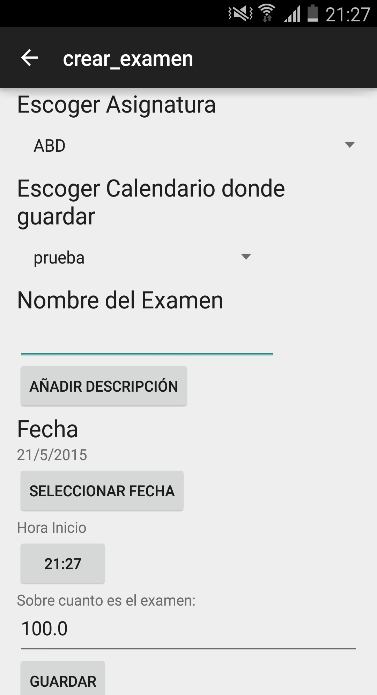
\includegraphics{figs/crearExamen.png}} 
    \caption{Actividad Crear Examen} 
    \label{fig:crearExamen} 
  \end{center} 
\end{figure}
Para terminar el formulario, el usuario tendrá que poner sobre cuánto se evaluará ese examen, siendo como valor por defecto la nota máxima de la asignatura y el valor mínimo cero.
Hay dos formas en las que se podrá guardar un examen:
1) En local: Si el usuario no dispone de Internet, la lógica de negocio hará que se cree el examen en la base de datos únicamente.
2) En Ambos: Si el usuario dispone de Internet, se creará un evento de examen en el calendario de Google escogido  y se almacenará también en la base de datos.

En la actividad de \textbf{Ver lista de exámenes}, funciona de la siguiente manera: El módulo encargado de mostrar la lista de exámenes genera una lista mediante la clase ExpandableList de Android, este tipo de lista agrupa el tipo de objeto que se quiere guardar, con una condición que hay que especificar al crear la lista. Al crearse la lista cada elemento, tendrá  sublistas dentro que tendrán una relación de filial con el elemento de la lista principal. Para agrupar los exámenes, se ha escogido la asignatura como categoría de agrupación dentro de la lista, para hacerla más legible y más ordenada.

Se puede modificar un examen manteniéndolo pulsado, esto hará que aparezca un menú y ahí se podrá seleccionar la opción de editar.

El caso de uso de \textbf{Modificar Examen} tiene el siguiente uso: si se desea modificar un examen se puede entrar mediante el caso de uso explicado anteriormente o desde la opción de ver examen. De las dos formas, el usuario acabará en una actividad nueva donde se le mostrará los campos del examen para modificar, y podrá cambiarlos todos excepto el nombre del examen.
Aparte de modificar datos del objeto examen, también se podrá acceder al caso de uso de modificar nota, que estará ligada a modificar examen cuando se guarde el examen.

\textbf{Ver examen}, este caso de uso es muy parecido al caso de uso de ver asignatura, donde mostrarán los campos del examen que se quieren ver. También dará acceso a los casos de uso de Modificar Examen y Borrar examen.

Para acabar los casos de uso referentes a examen tenemos \textbf{Borrar Examen}: este caso de uso trata de realizar el borrado de un examen tanto de la base de datos del dispositivo como de Google Calendar. En el caso que Google Calendar presente algún fallo sólo lo borrará de manera local, y será el usuario quien tendrá que borrar el evento del Google Calendar.
A este caso de uso se llega desde la actividad de ver examen, y es un botón al final del layout.

\subsubsection{Casos de uso sobre Nota}
\label{subsubsecc:Casos de uso sobre Nota}

Tanto el caso de uso \textbf{Modificar nota asignatura}, como el caso de uso \textbf{Modificar nota examen}, son casos de uso transparentes para el usuario porque no hay un botón como tal para llegar, pero el usuario lo realiza cuando quiere explícitamente modificar las notas de cada objeto metiéndose en la modificación del objeto en cuestión.
Estos casos de uso trabajan sobre el objeto Nota, los dos casos de uso modifican el valor integer que está guardado en la base de datos de cada tabla. En el caso de la asignatura sólo tendrá que coger el identificador de la asignatura y cambiar el valor, en cambio, en modificar nota examen la tarea se complica ya que las notas no están dentro del objeto examen, sino que hay una tabla donde se conectan la nota de un examen que pertenece a una asignatura. Así que para ello, hay que buscar en la tabla el examen y la asignatura que se quiere modificar y cambiar la nota.

\subsubsection{Casos de uso generales}
\label{subsubsecc:Casos de uso generales}

Dentro de los casos de uso generales se hablará sobre los casos de uso que se pueden realizar sin estar usando los objetos que se han trabajado en el proyecto, la mayoría son casos de uso relacionados con APIs de Google o solamente son pantallas de ayuda para el usuario.

Para empezar el caso de uso fundamental, si se quieren usar los servicios de Google, \textbf{Escoger cuenta de Google}, en este caso de uso, el usuario podrá escoger qué cuenta usará tanto para el Google Calendar, donde cogerá los calendarios para crear los exámenes, y aparte la cuenta donde se quiere guardar el backup de la base de datos.

\textbf{Casos de uso vinculados a Google Calendar}, estos casos de uso son muy variados y son los que Google pone como ejemplo a la hora de usar Google Calendar. Se dejaron en la aplicación ya que son útiles a la hora de realizar modificaciones en los calendarios de Google sin tener que estar metiéndose expresamente.
Alguno de los casos de uso vinculados son, la creación de un calendario, ver la lista de los calendarios, modificar un calendario, borrar un calendario, y triplicar un calendario. También permite la opción de visualizar un calendario, donde sí se usa la opción se mostrará el nombre del calendario y dará la posibilidad de modificarlo.

\textbf{Casos de uso vinculados a Google Drive}, para la realización del backup se usa el API de Google Drive, hay dos casos principales: exportar e importar la base de datos.
En el caso de uso de exportar, el usuario escoge la carpeta donde quiere guardar la base de datos y también se le permite la opción de crear una carpeta nueva.
Después el usuario pulsara el botón de exportar base de datos para que se realice una copia en Google Drive de la base de datos en ese momento.
Para el caso de uso de importar el funcionamiento es muy parecido, el usuario selecciona la base de datos que quiere importar y una vez que tiene seleccionado el fichero, sólo tiene que darle al botón para realizar el borrado de la antigua base de datos y la copia al dispositivo de la guardada.

\textbf{Caso de uso ver información de ayuda},este caso de uso se incluyó para que los Baldusers pudieran ponerse en contacto conmigo de forma rápida en el caso de que no tuvieran mi número de teléfono o mi email, también se les facilitó la URL de la carpeta donde estarían los ficheros de feedback que tenían que rellenar.

\subsection{Modelo de datos}
\label{subsecc:modelo de datos}

La aplicación Android guarda los datos en el dispositivo, tanto la base de datos como las preferencias.
Los datos que se guardan como preferencias son los relativos a la autenticación y los ajustes. El encargado de almacenar esta información es el método SharedPreferences de Android, almacena la información en formato XML.


\begin{figure}[H]
  \begin{center} 
    \scalebox{0.8}{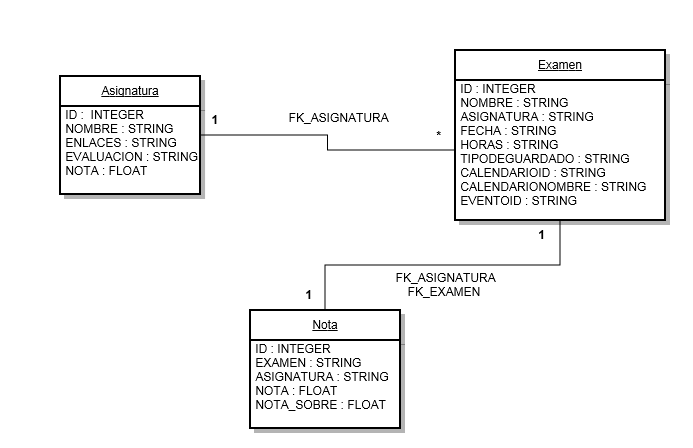
\includegraphics{figs/modeloRelacional.png}} 
    \caption{Modelo relacional} 
    \label{fig:ModeloRelacional} 
  \end{center} 
\end{figure}
La base de datos trabaja con distintos tipos de datos, siendo el más abundante el tipo string.
Los datos sobre los que trabajara la base de datos serán los siguientes:

\textbf{Asignatura}: Representa a la asignatura que está matriculado el usuario, y es la clase de la que depende examen. Tiene el nombre de la asignatura, una  lista de enlaces para la asignatura  y el tipo de evaluación (Continua o Conjunta).

\textbf{Examen}: Es cada evento que desea apuntar el usuario en una asignatura, tiene relación con nota. Guarda la información del nombre, descripción, fecha, hora y la asignatura.

\textbf{Nota}: Cada examen tiene una nota asociada, y este objeto guarda la información de la nota del examen como la nota total que se puede sacar en la asignatura.
Estas 3 clases son los principales objetos de la aplicación, y todos los casos de uso giran en torno a ellas.
La relación es la siguiente:



\subsection{Interfaces de usuario}
\label{subsecc:Interfaces de usuario}

En Android se usan las Activities para implementar las interfaces de usuario, estas contienen la lógica y controlan su ciclo de vida.
Las Activities usadas en Baldugenda son las siguientes: AcitividadPrincipal, Asignatura, crear\_asignatura, modificar\_asignatura, lista\_asignaturas, Examen, crear\_examen, modificar\_examen, lista\_exámenes, Drive, contacto.

\textbf{Actividad Principal}

Es la primera ventana que ve el usuario y en ella se muestran todas las opciones que puede hacer mediante iconos.
Desde esta actividad puede ir a cualquier  caso de uso.

\textbf{Crear Asignatura}

Es la actividad que muestra el formulario que se tiene que rellenar para crear una asignatura.

\textbf{Modificar Asignatura}

Esta interfaz muestra los valores de la asignatura escogida y la posibilidad de modificarlos y guardar de nuevo la asignatura.

\textbf{Lista asignaturas}

Esta interfaz muestra la lista de las asignaturas que se encuentran creadas en la base de datos.
También permite la posibilidad mediante la pulsación larga en cada asignatura de ir al caso de uso de borrar o editar la asignatura escogida.

\textbf{Asignatura}

Muestra los valores de la asignatura y permite la posibilidad de acceder al caso de uso de borrar y editar asignatura.

\textbf{Crear Examen}

Muestra el formulario que se tiene que rellenar para crear un examen.

\textbf{Modificar Examen}

Esta interfaz muestra los valores del examen escogido, la posibilidad de modificarlos y guardar de nuevo el examen.

\textbf{Lista exámenes}

Esta interfaz muestra la lista de los exámenes que se encuentran creados en la base de datos.
También permite la posibilidad mediante la pulsación larga en cada examen, de ir al caso de uso de editar el examen escogido.

\textbf{Examen}

Es la actividad que muestra los valores que tiene el examen escogido y nos permite acceder a los casos de uso de editar y borrar examen.
\newpage
\begin{figure}[H]
  \centering
  \begin{tikzpicture}[auto, node distance = 0.5cm and 0.5cm,every node/.style={inner sep=0pt}]
    \tikzset{A/.style={arrows={Circle-Stealth},draw,blue,ultra thick}}
    
    \node (main) {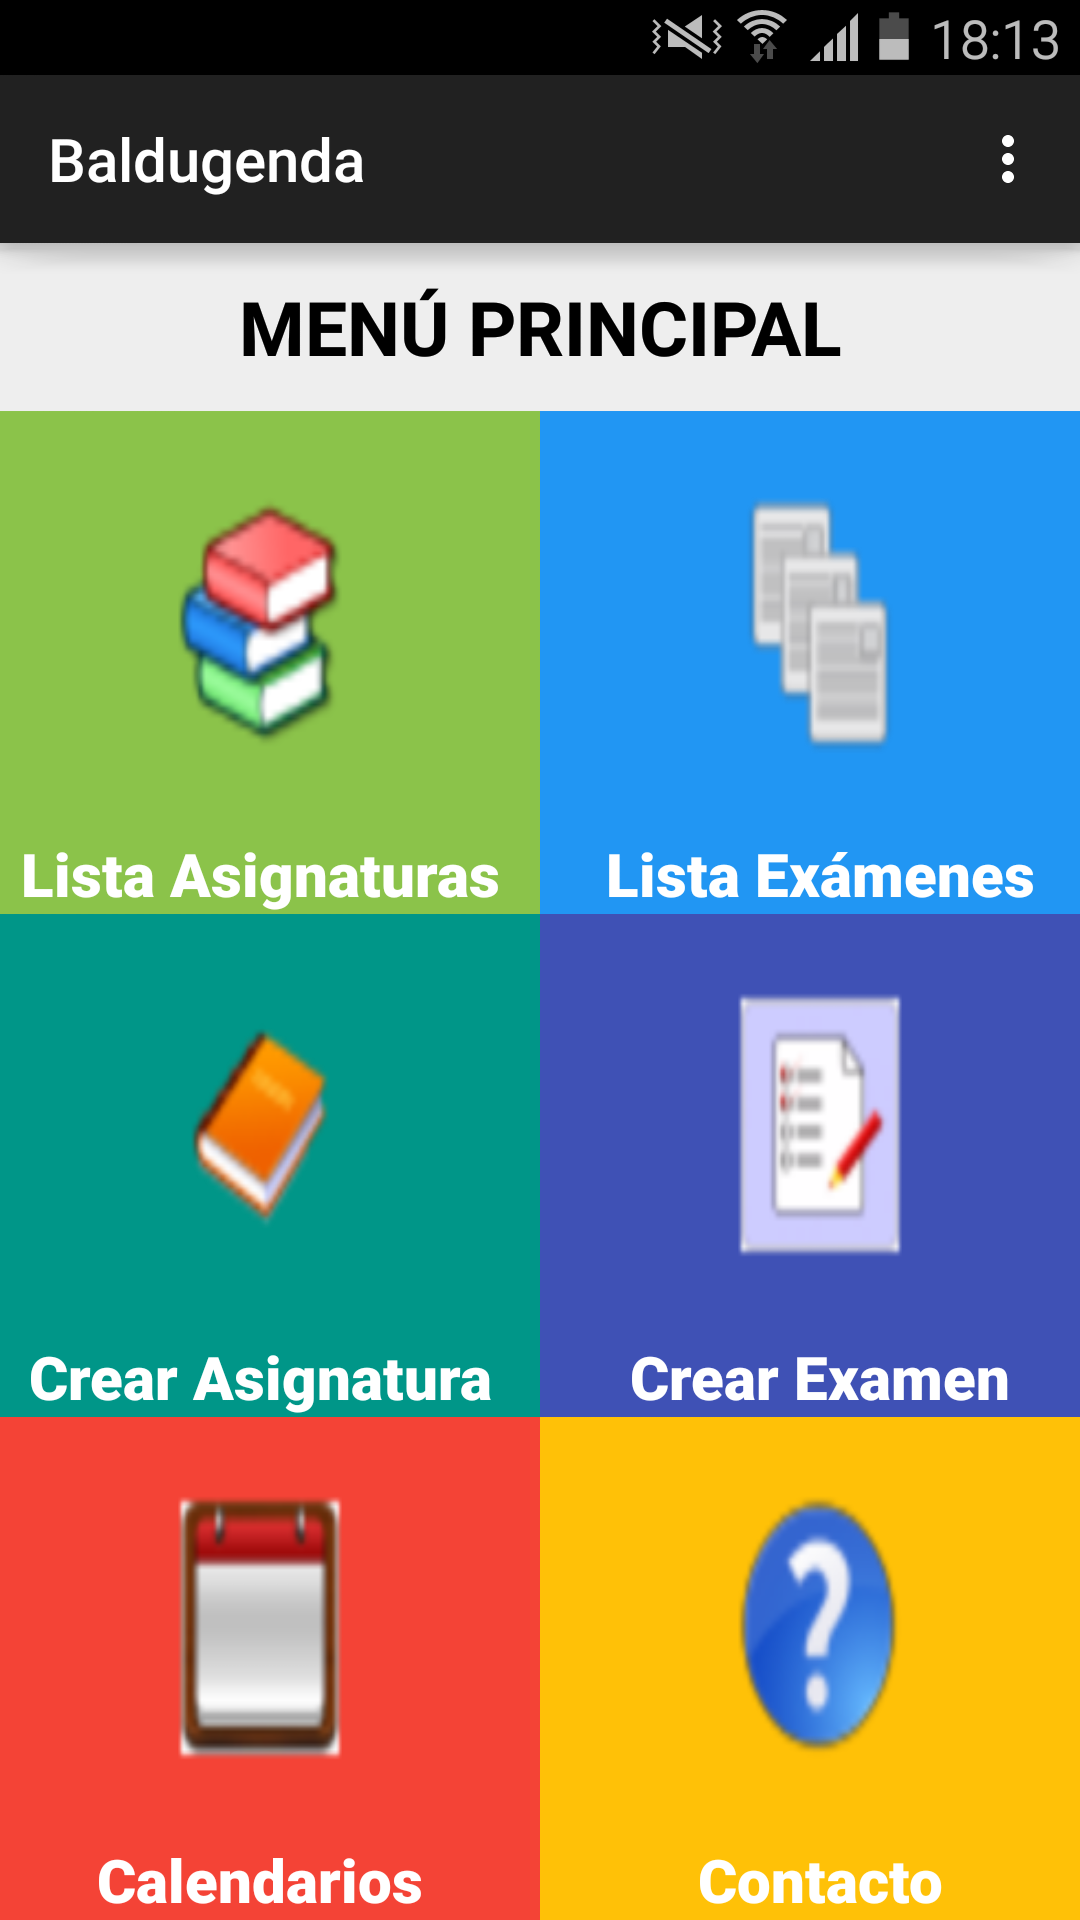
\includegraphics[width=3cm]{figs/capturas/1.png}};
	\node [left=of main] (crearAsignatura) {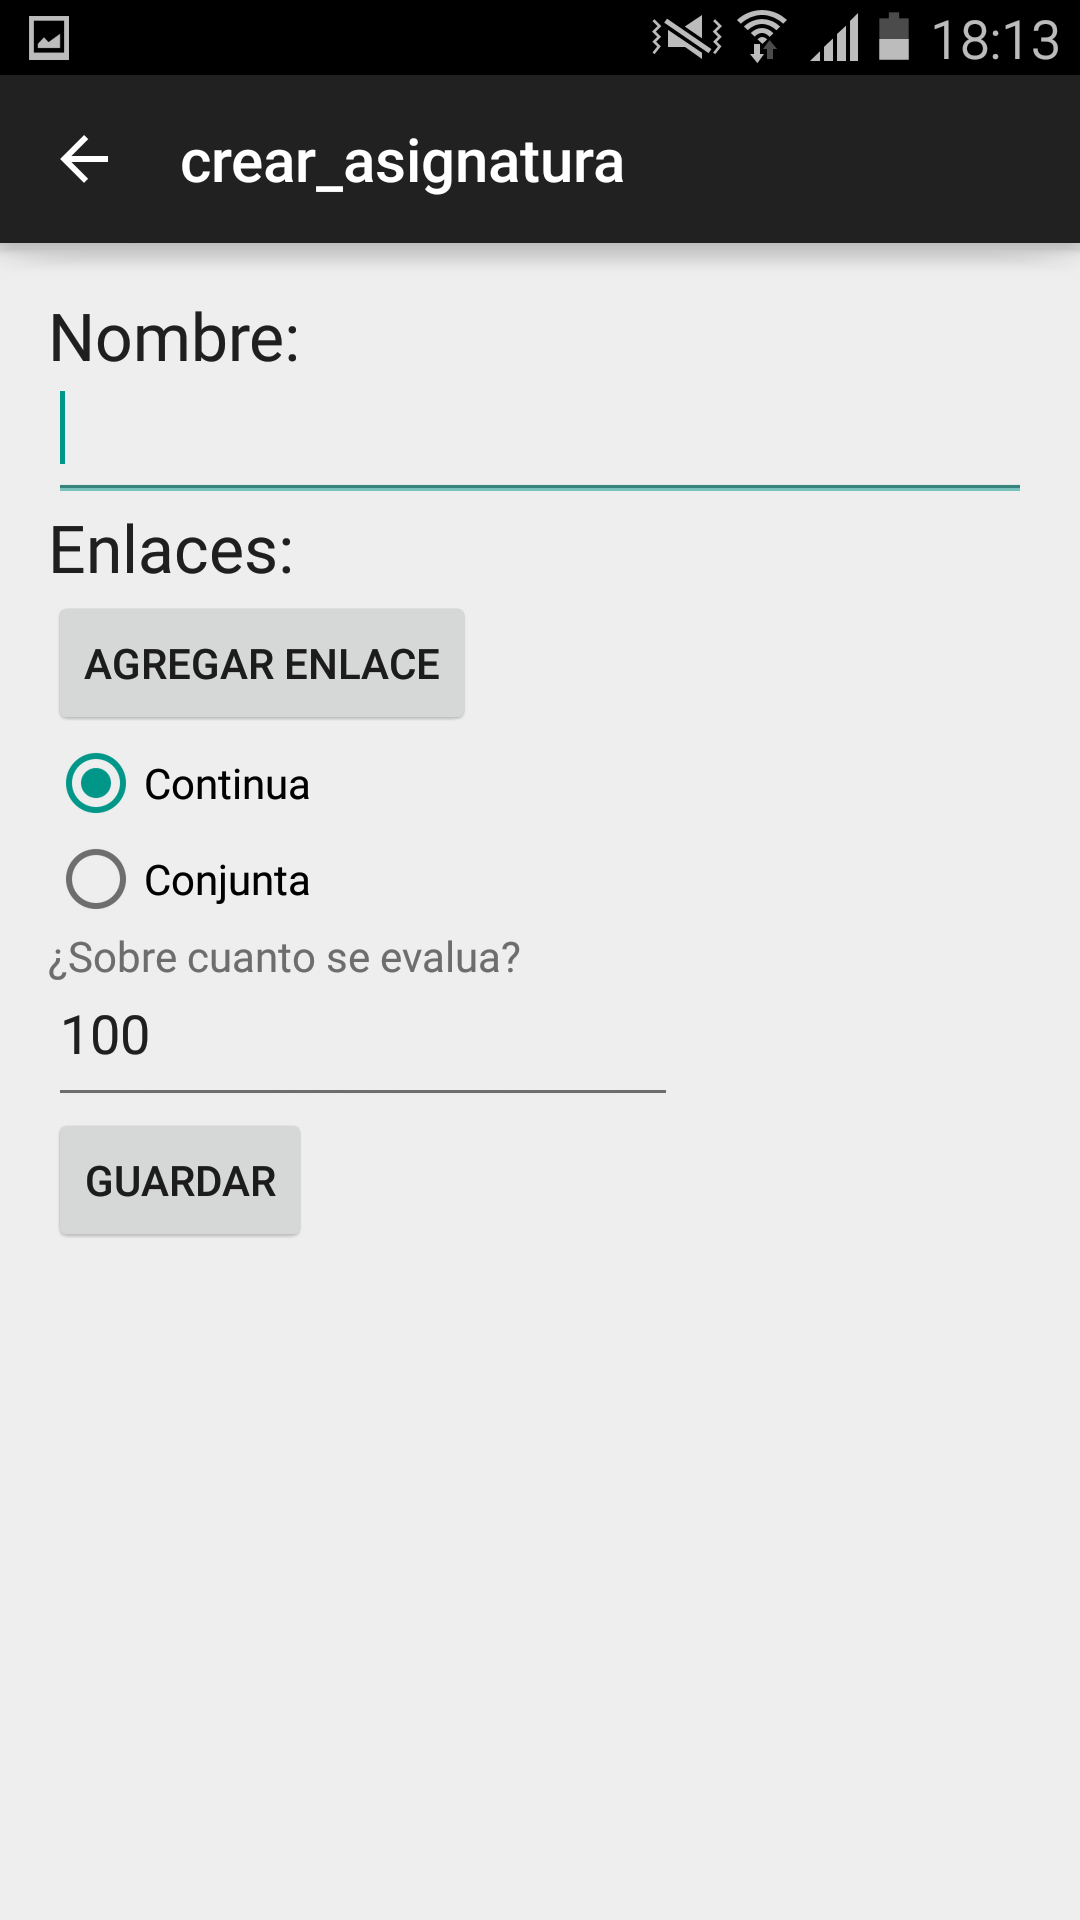
\includegraphics[width=3cm]{figs/capturas/3.png}};
    \node [left=of crearAsignatura] (asignatura) {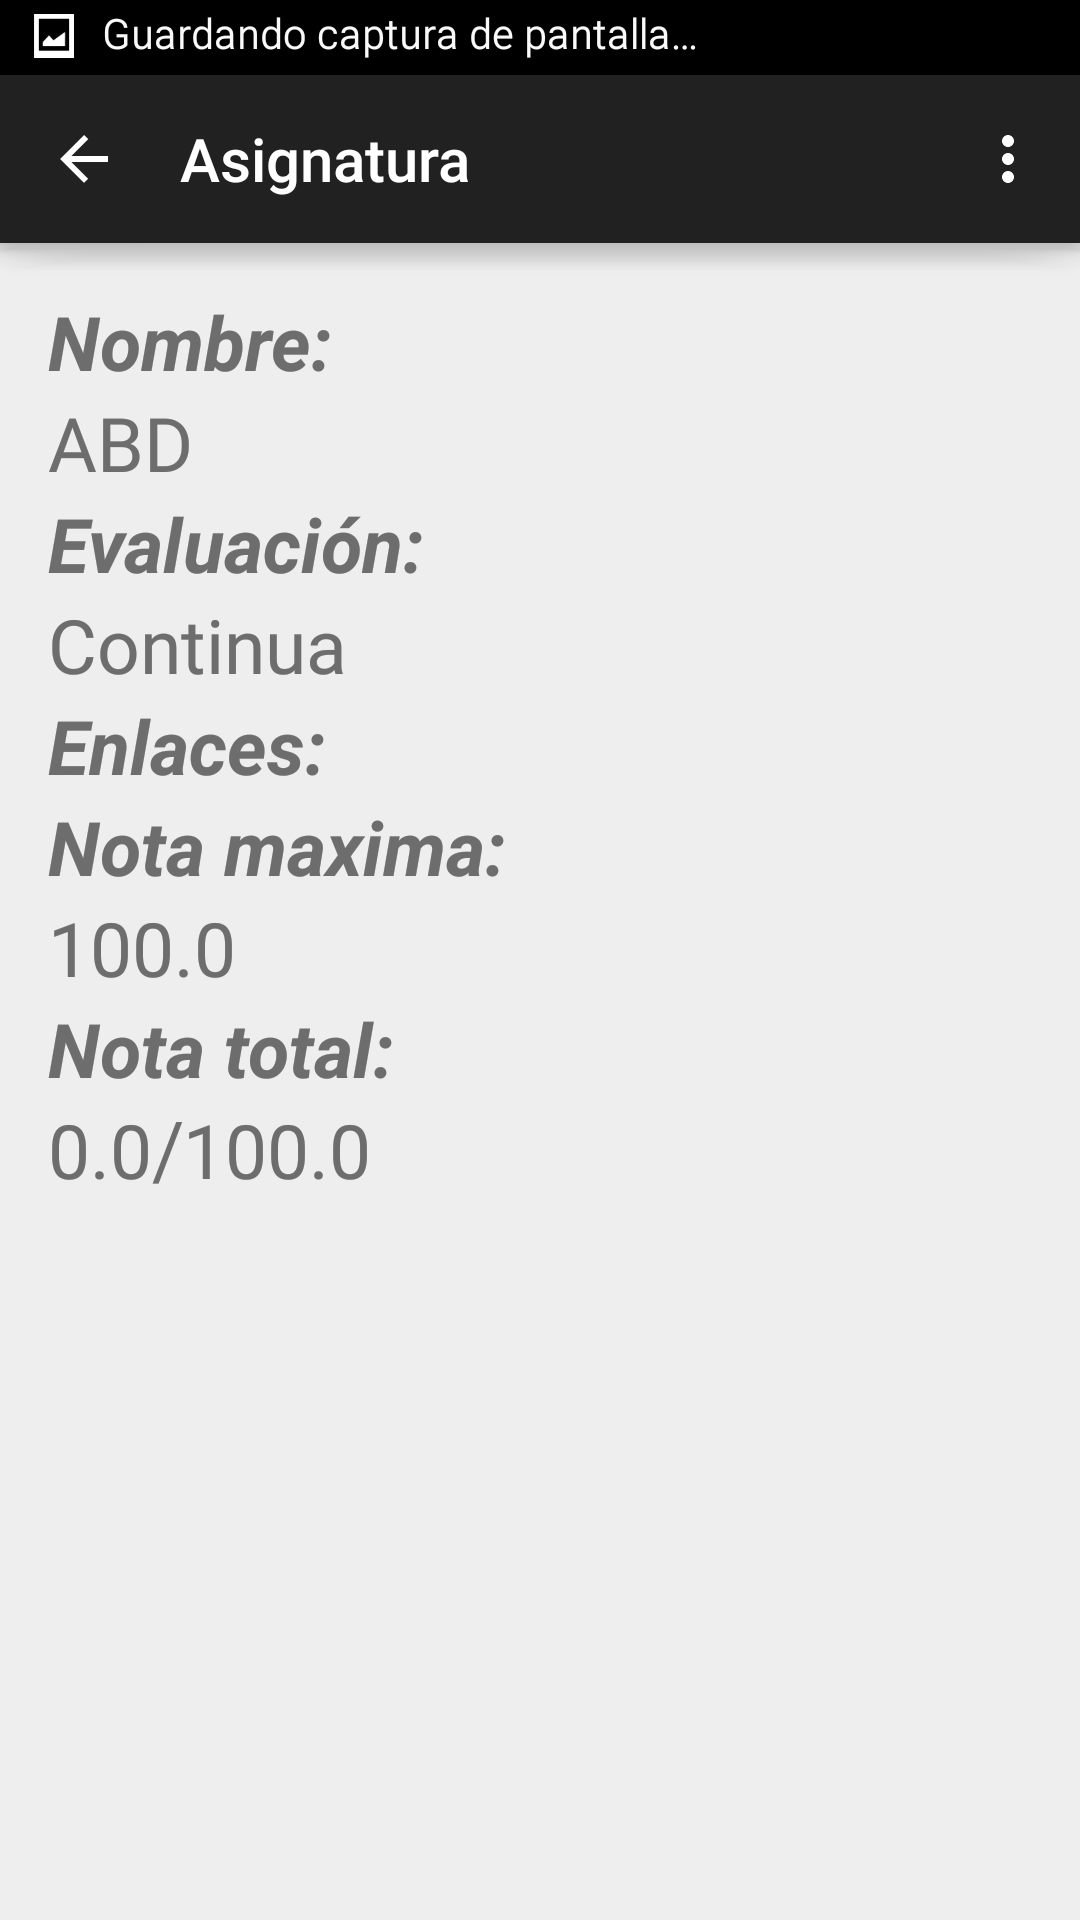
\includegraphics[width=3cm]{figs/capturas/6.png}};
    \node [right=of main] (examen) {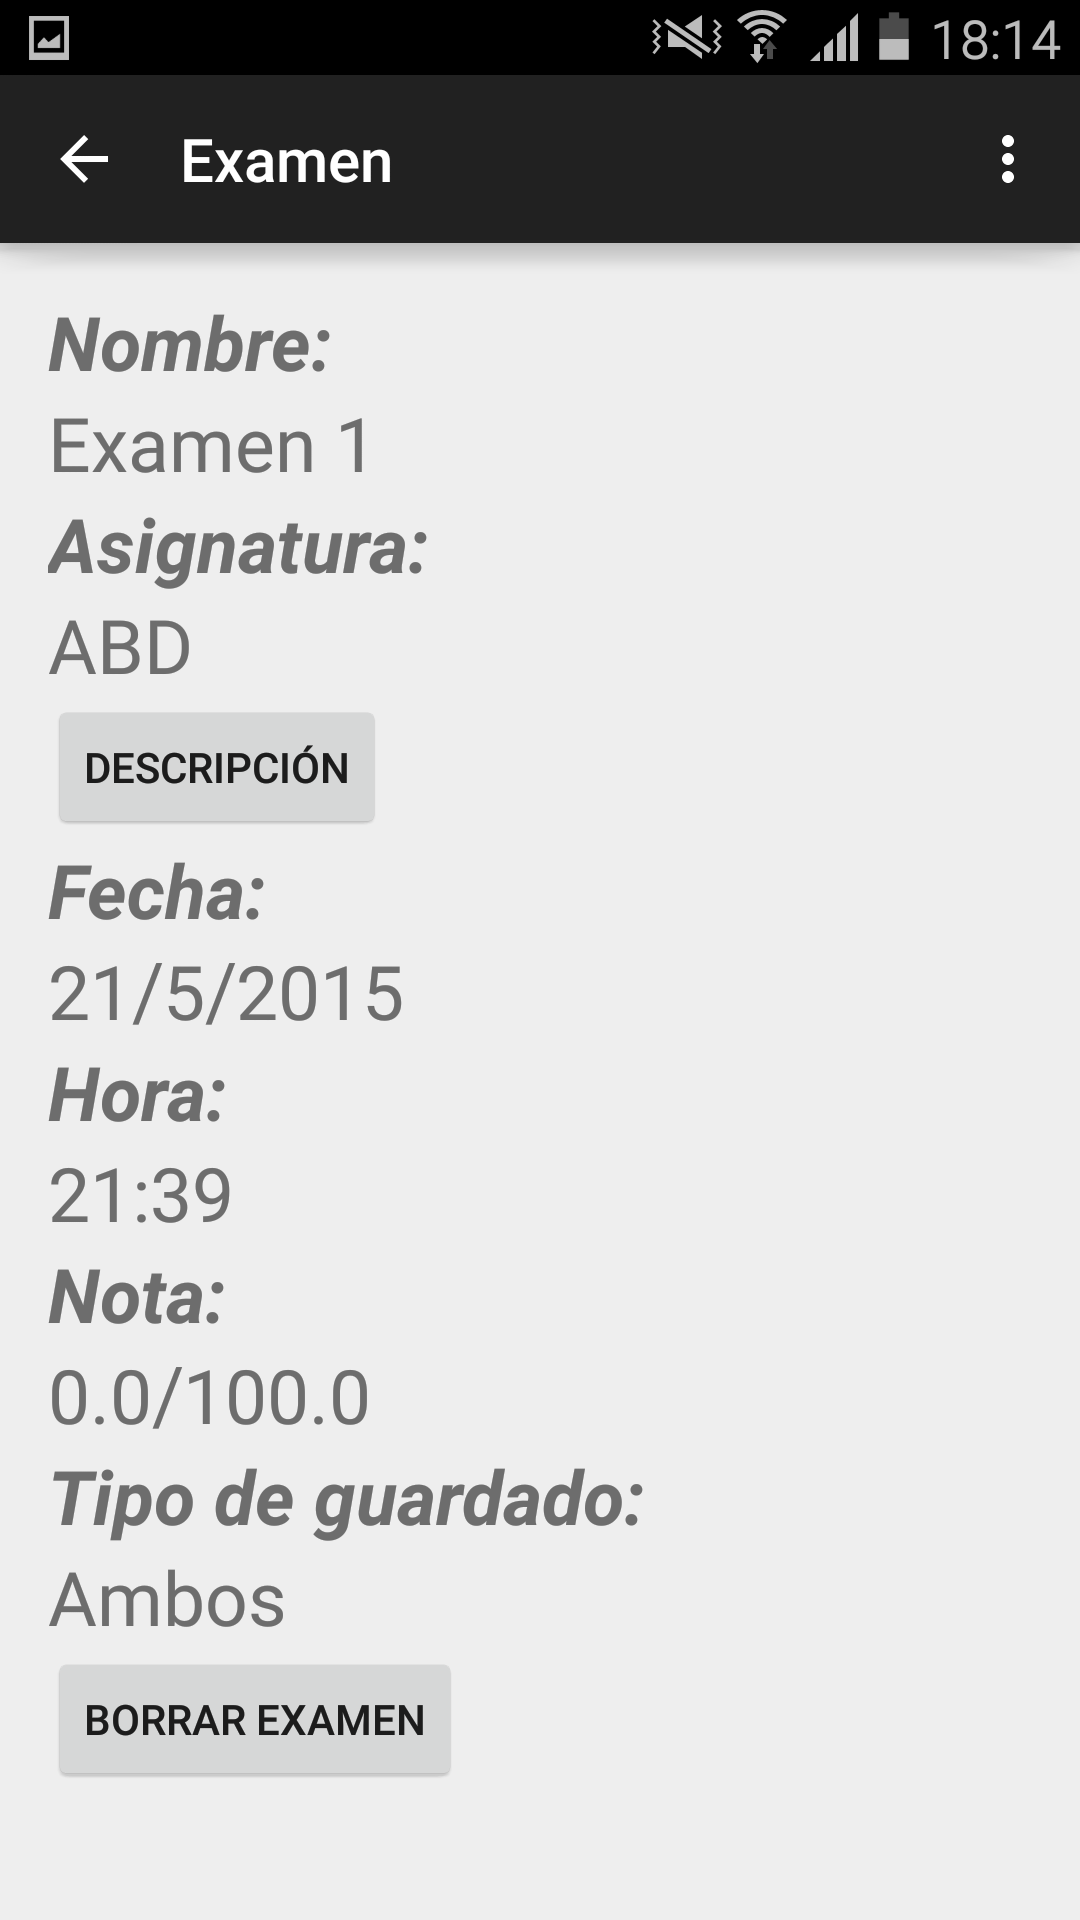
\includegraphics[width=3cm]{figs/capturas/7.png}};
    \node [below=of main] (backup) {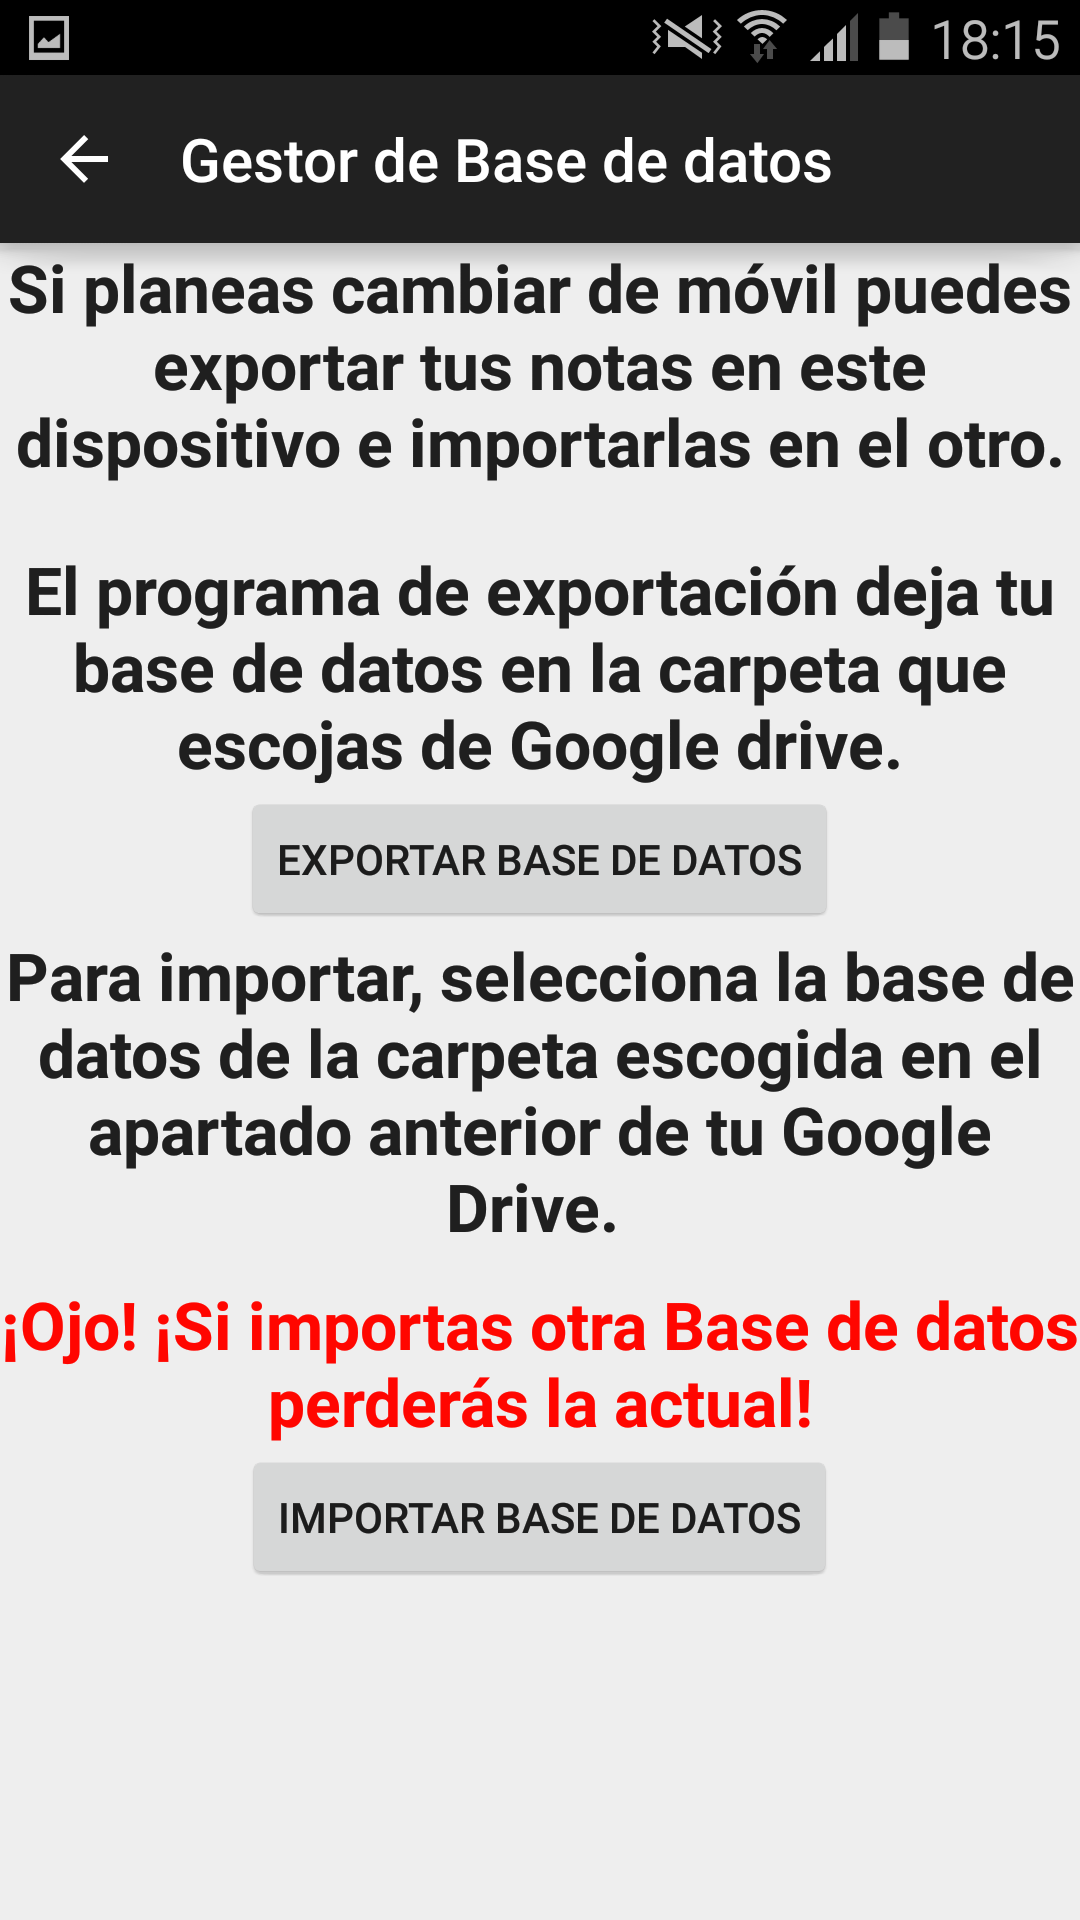
\includegraphics[width=3cm]{figs/capturas/11.png}};
    
	\node [above=of main] (listaExamen) {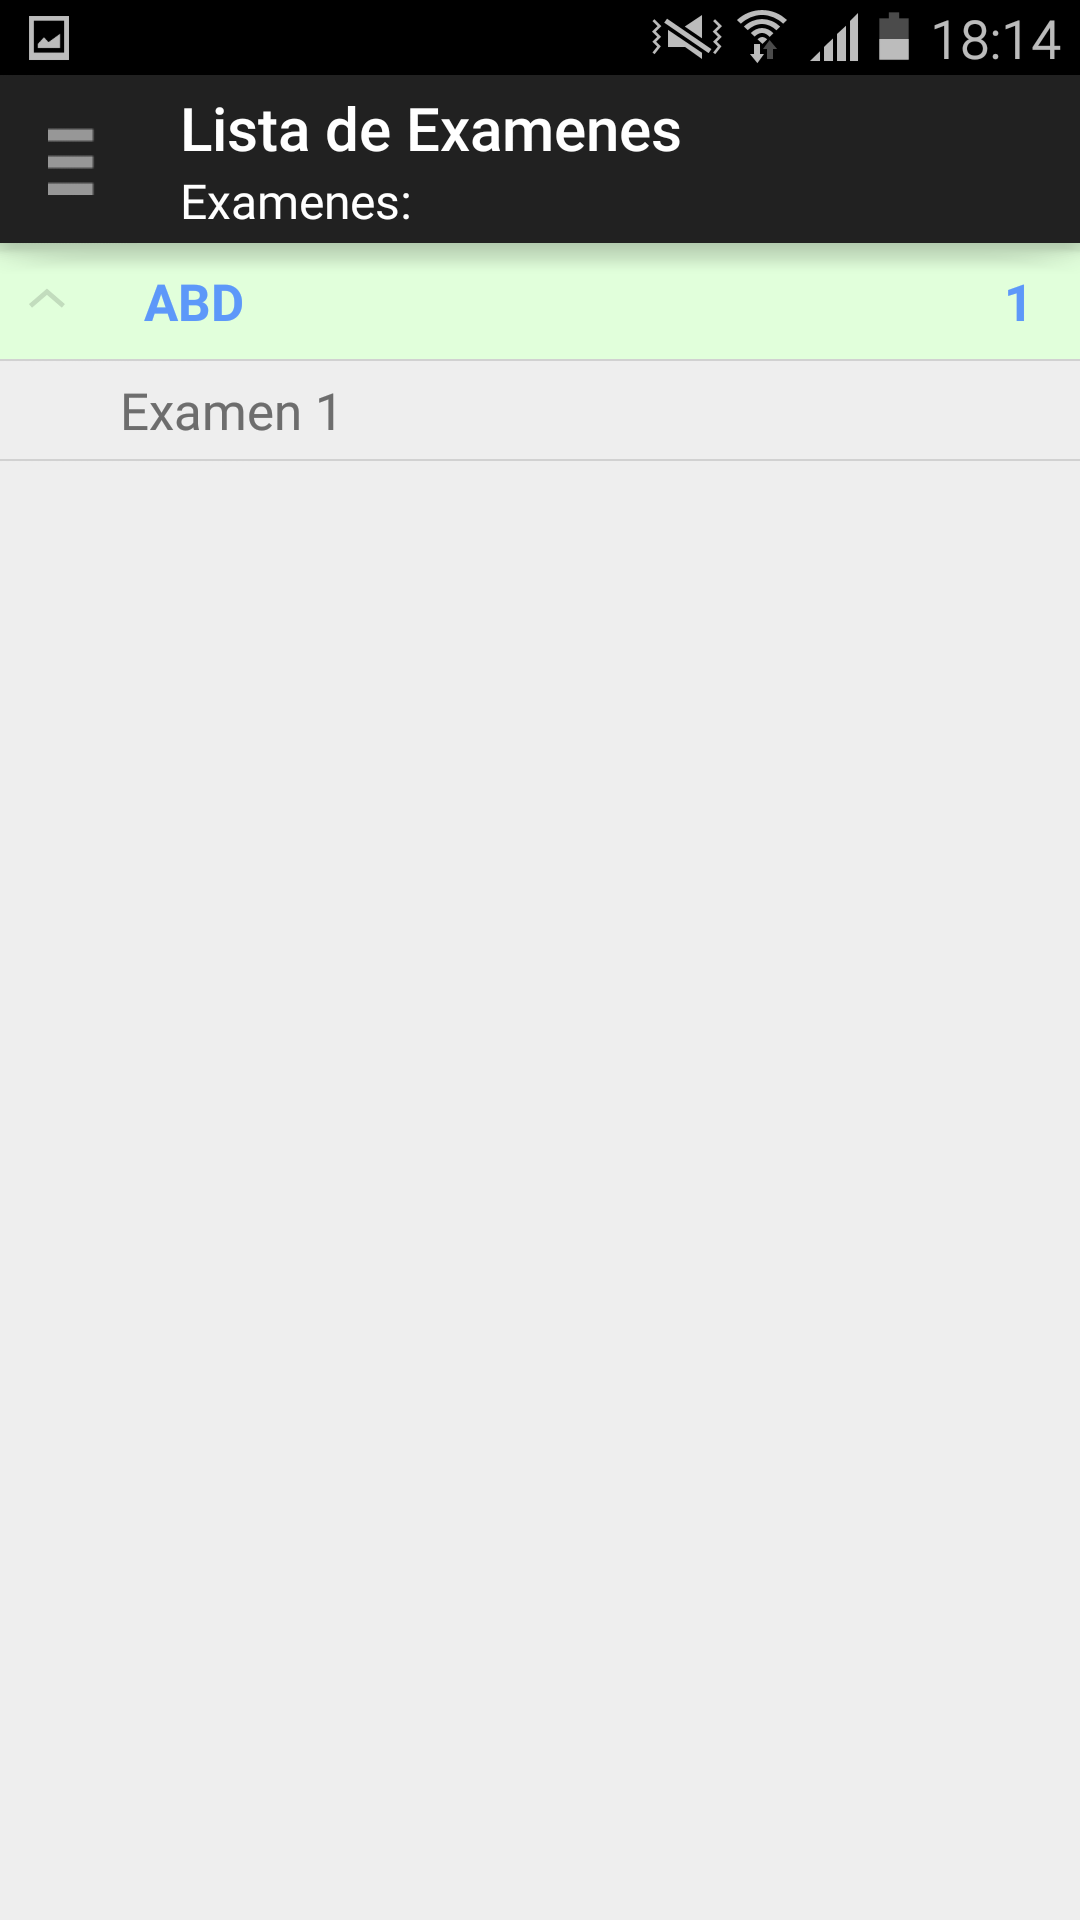
\includegraphics[width=3cm]{figs/capturas/4.png}};    
    
   	\node [left=of listaExamen] (listaAsignatura) {
\includegraphics[width=3cm]{figs/capturas/5.png}};
   	\node [left=of listaAsignatura] (modAsignatura) {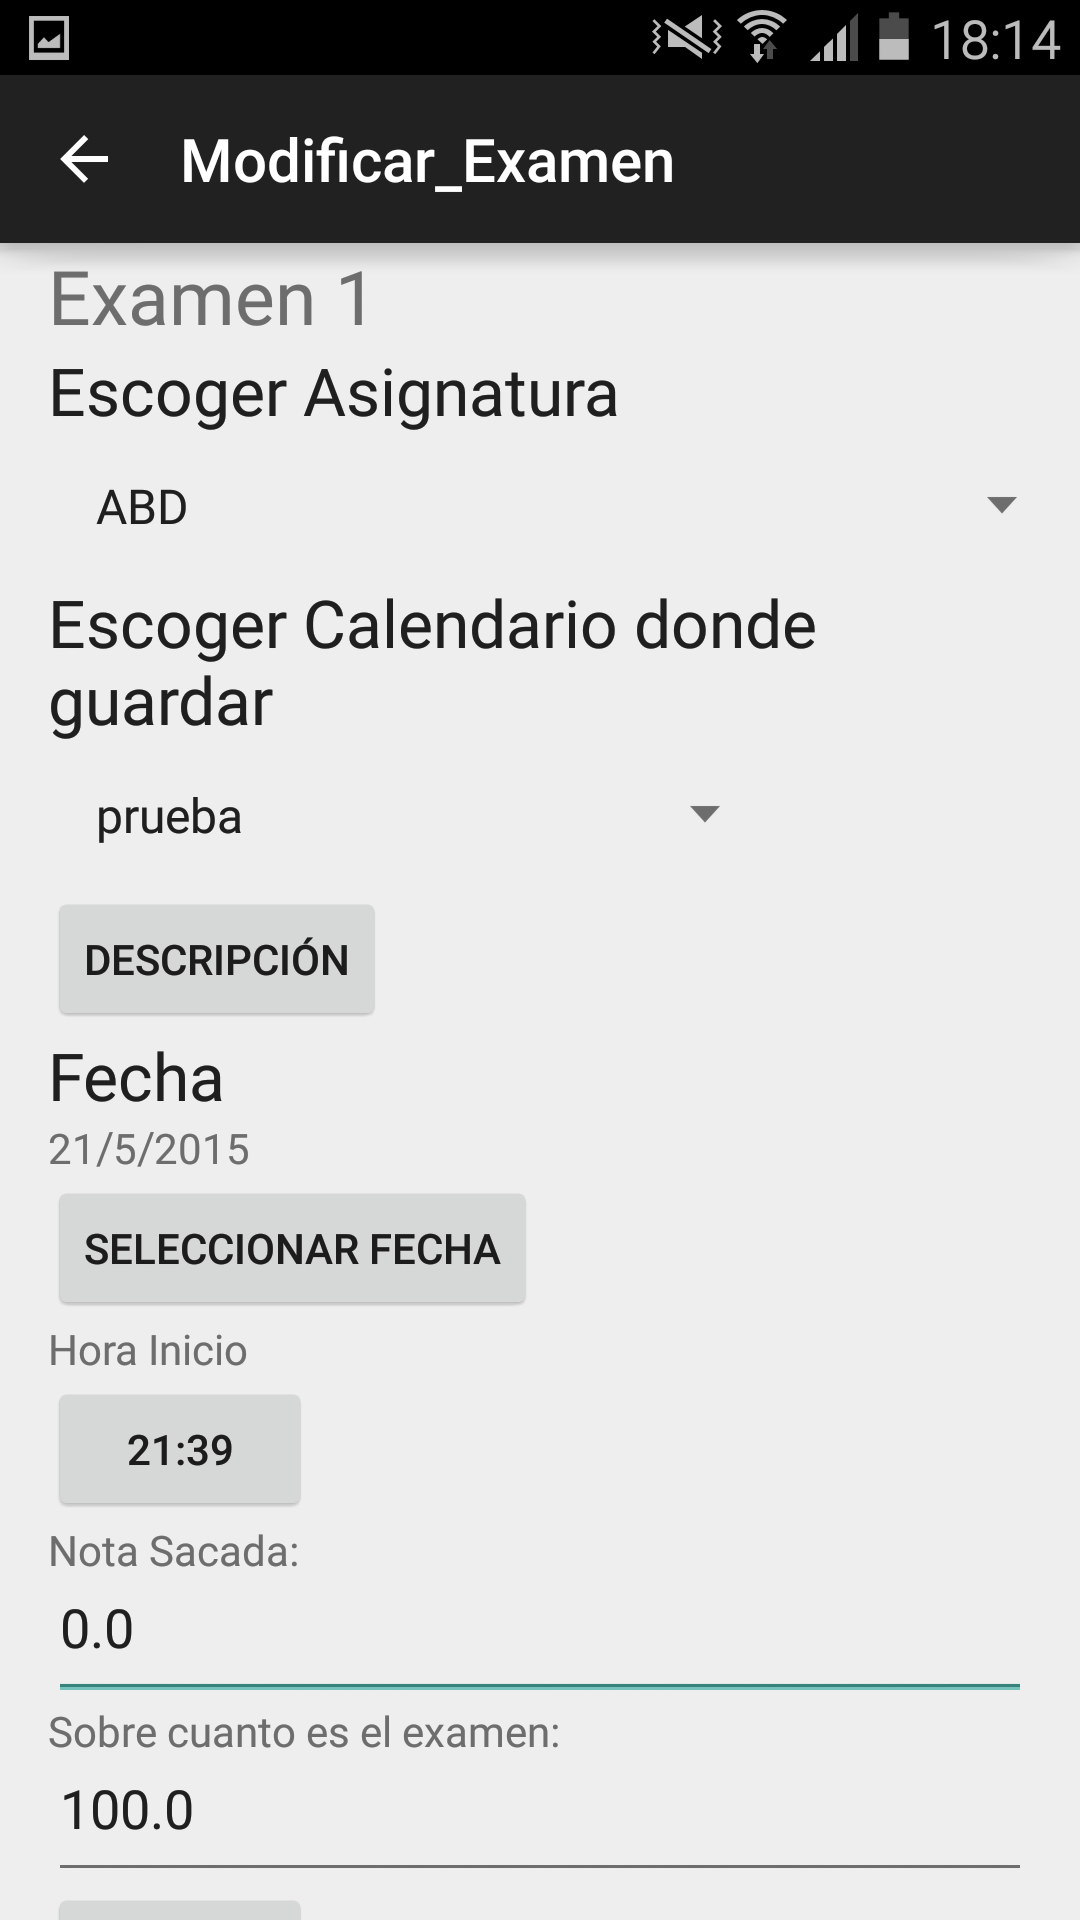
\includegraphics[width=3cm]{figs/capturas/8.png}};
    \node [right=of listaExamen] (modExamen) {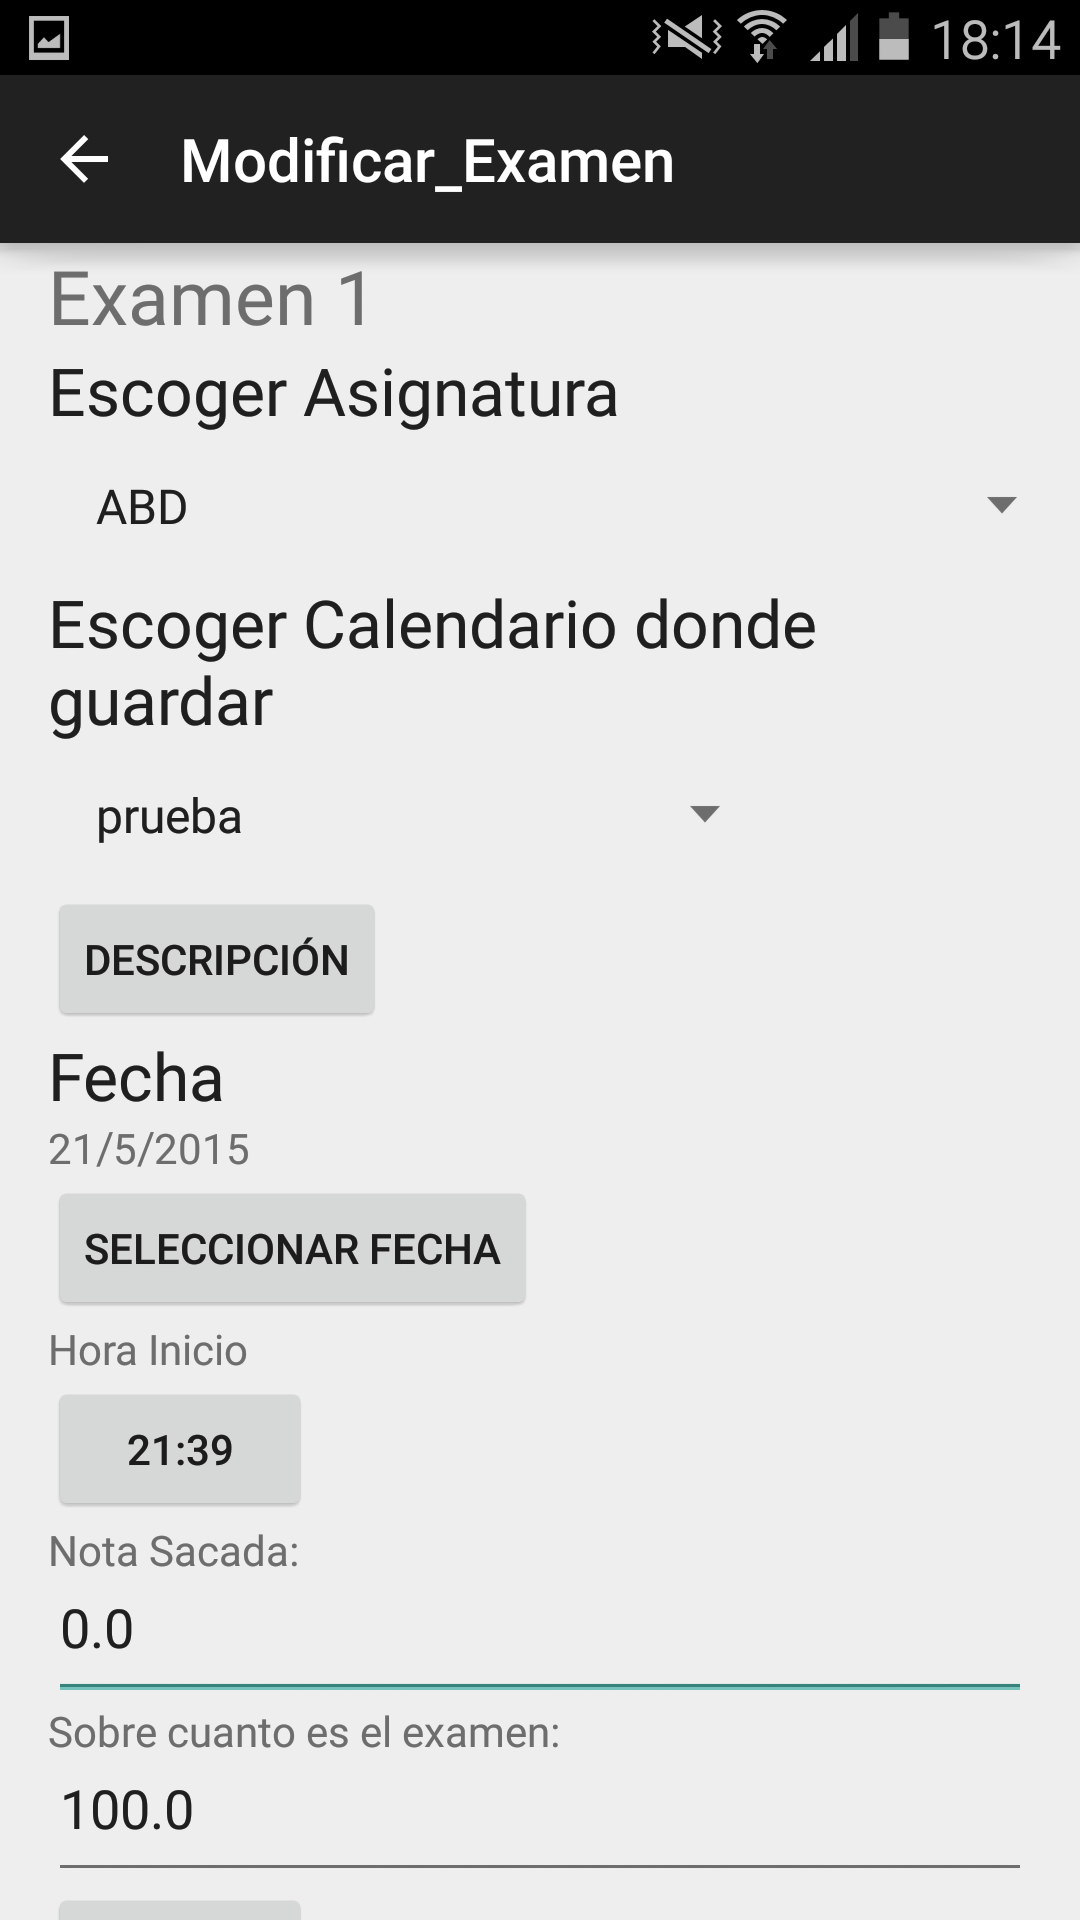
\includegraphics[width=3cm]{figs/capturas/8.png}}; 
    
    \node [left=of backup] (help) {
\includegraphics[width=3cm]{figs/capturas/14.png}};
    \node [left=of help] (calendar) {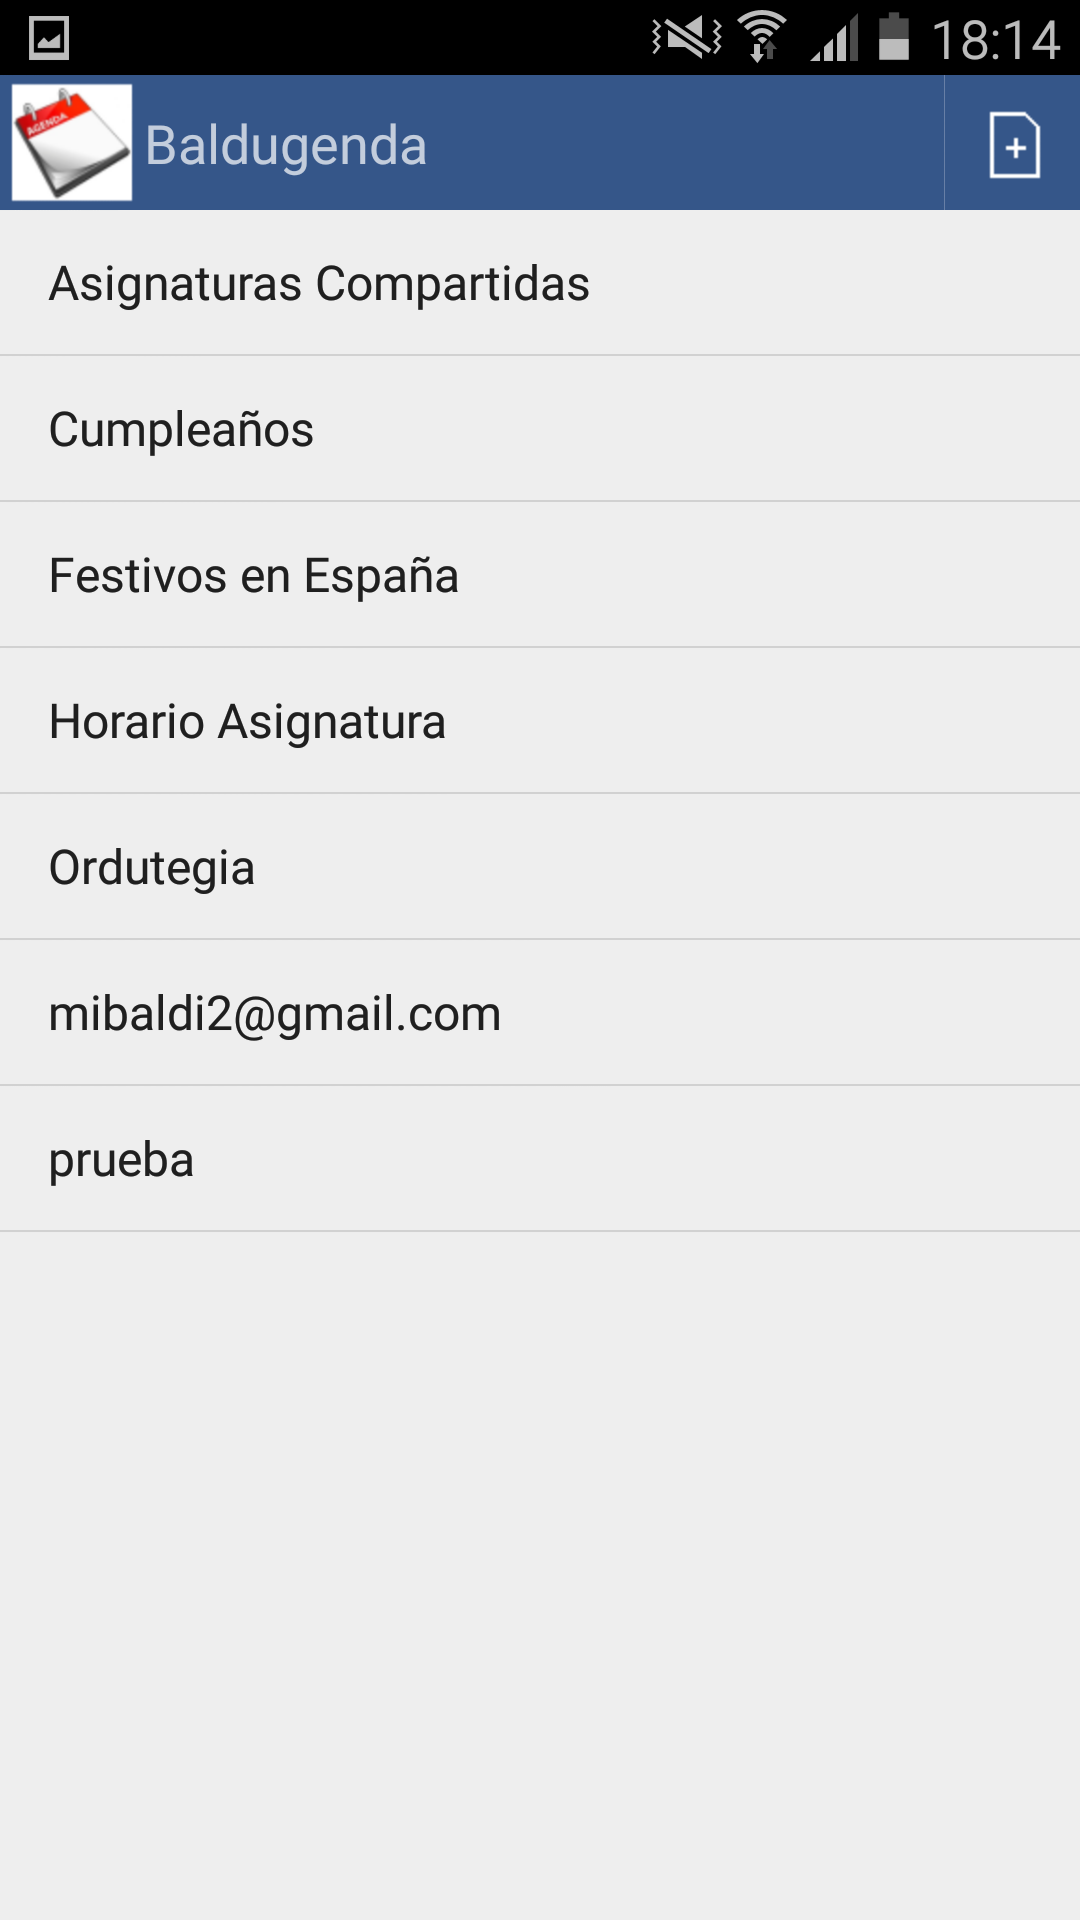
\includegraphics[width=3cm]{figs/capturas/10.png}};
    \node [right=of backup] (crearExamen) {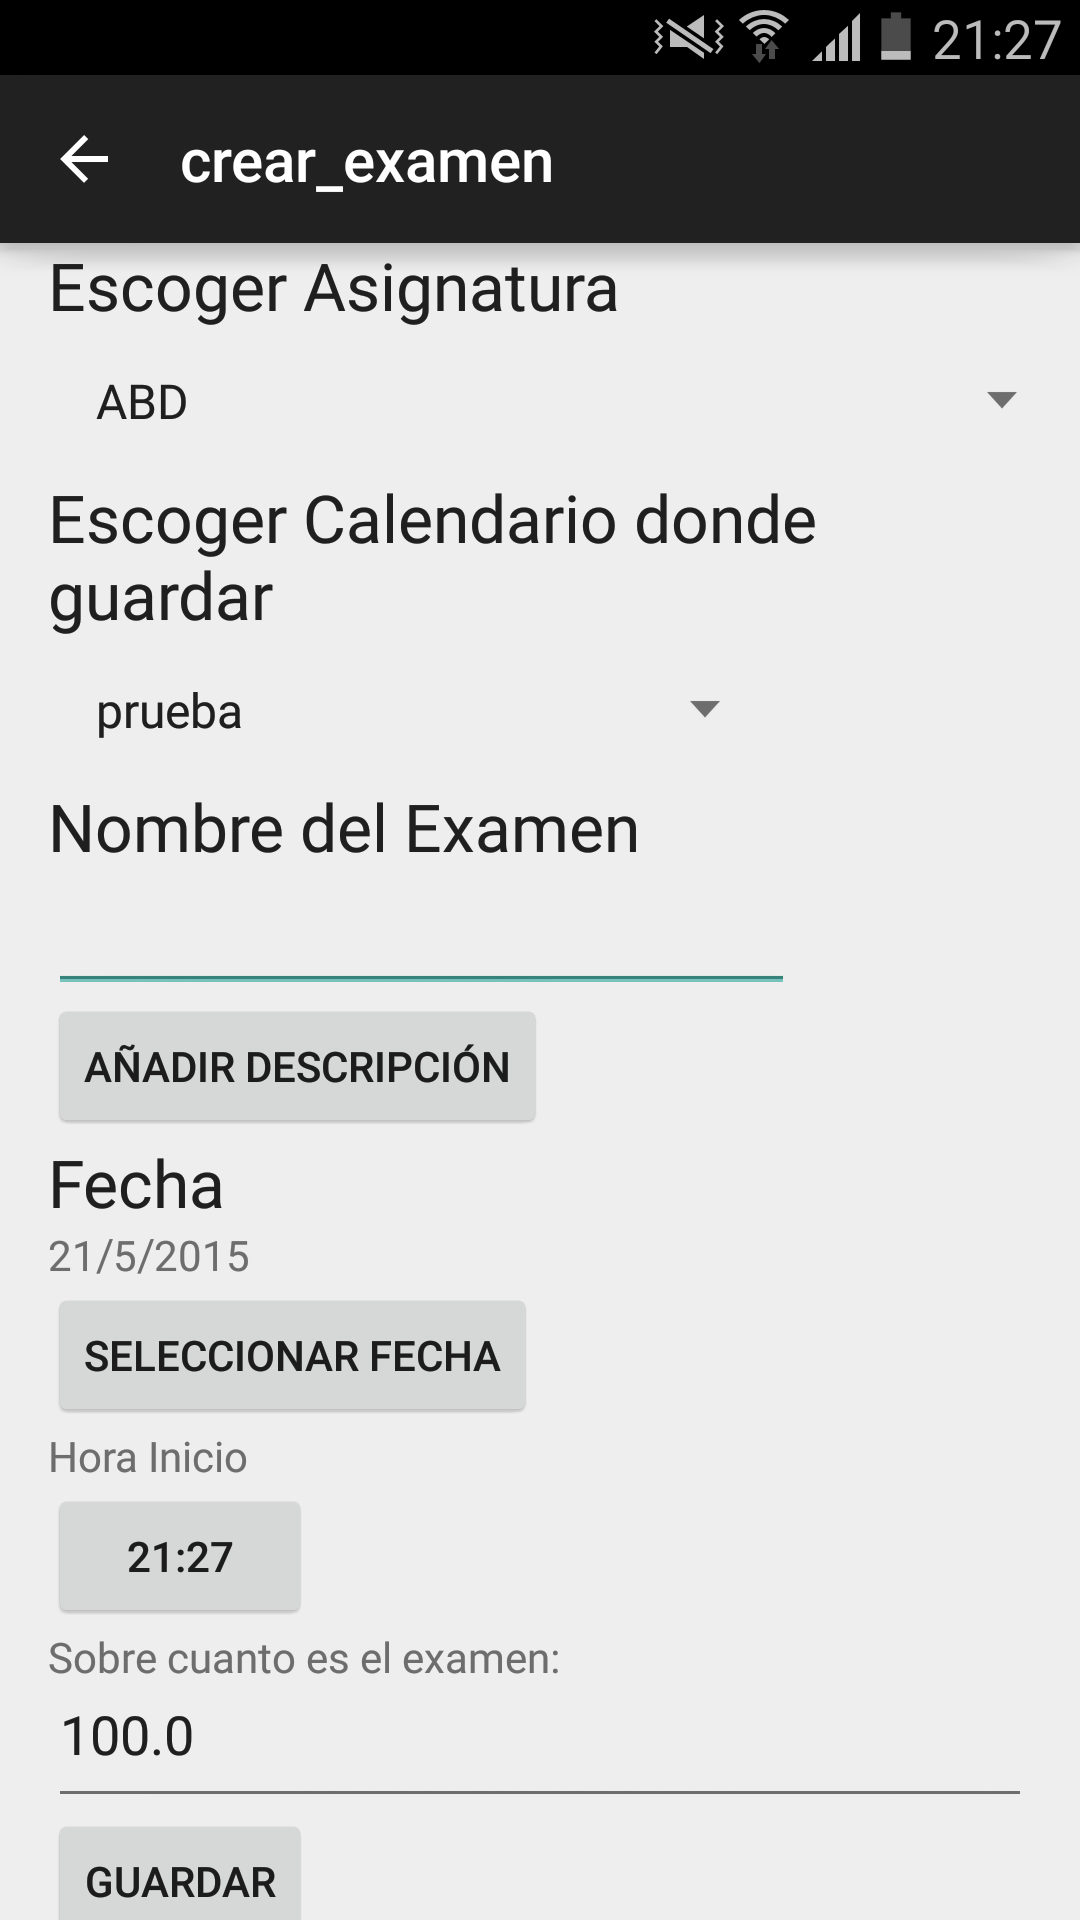
\includegraphics[width=3cm]{figs/capturas/2.png}}; 
    \node [below=of backup] (exportar) {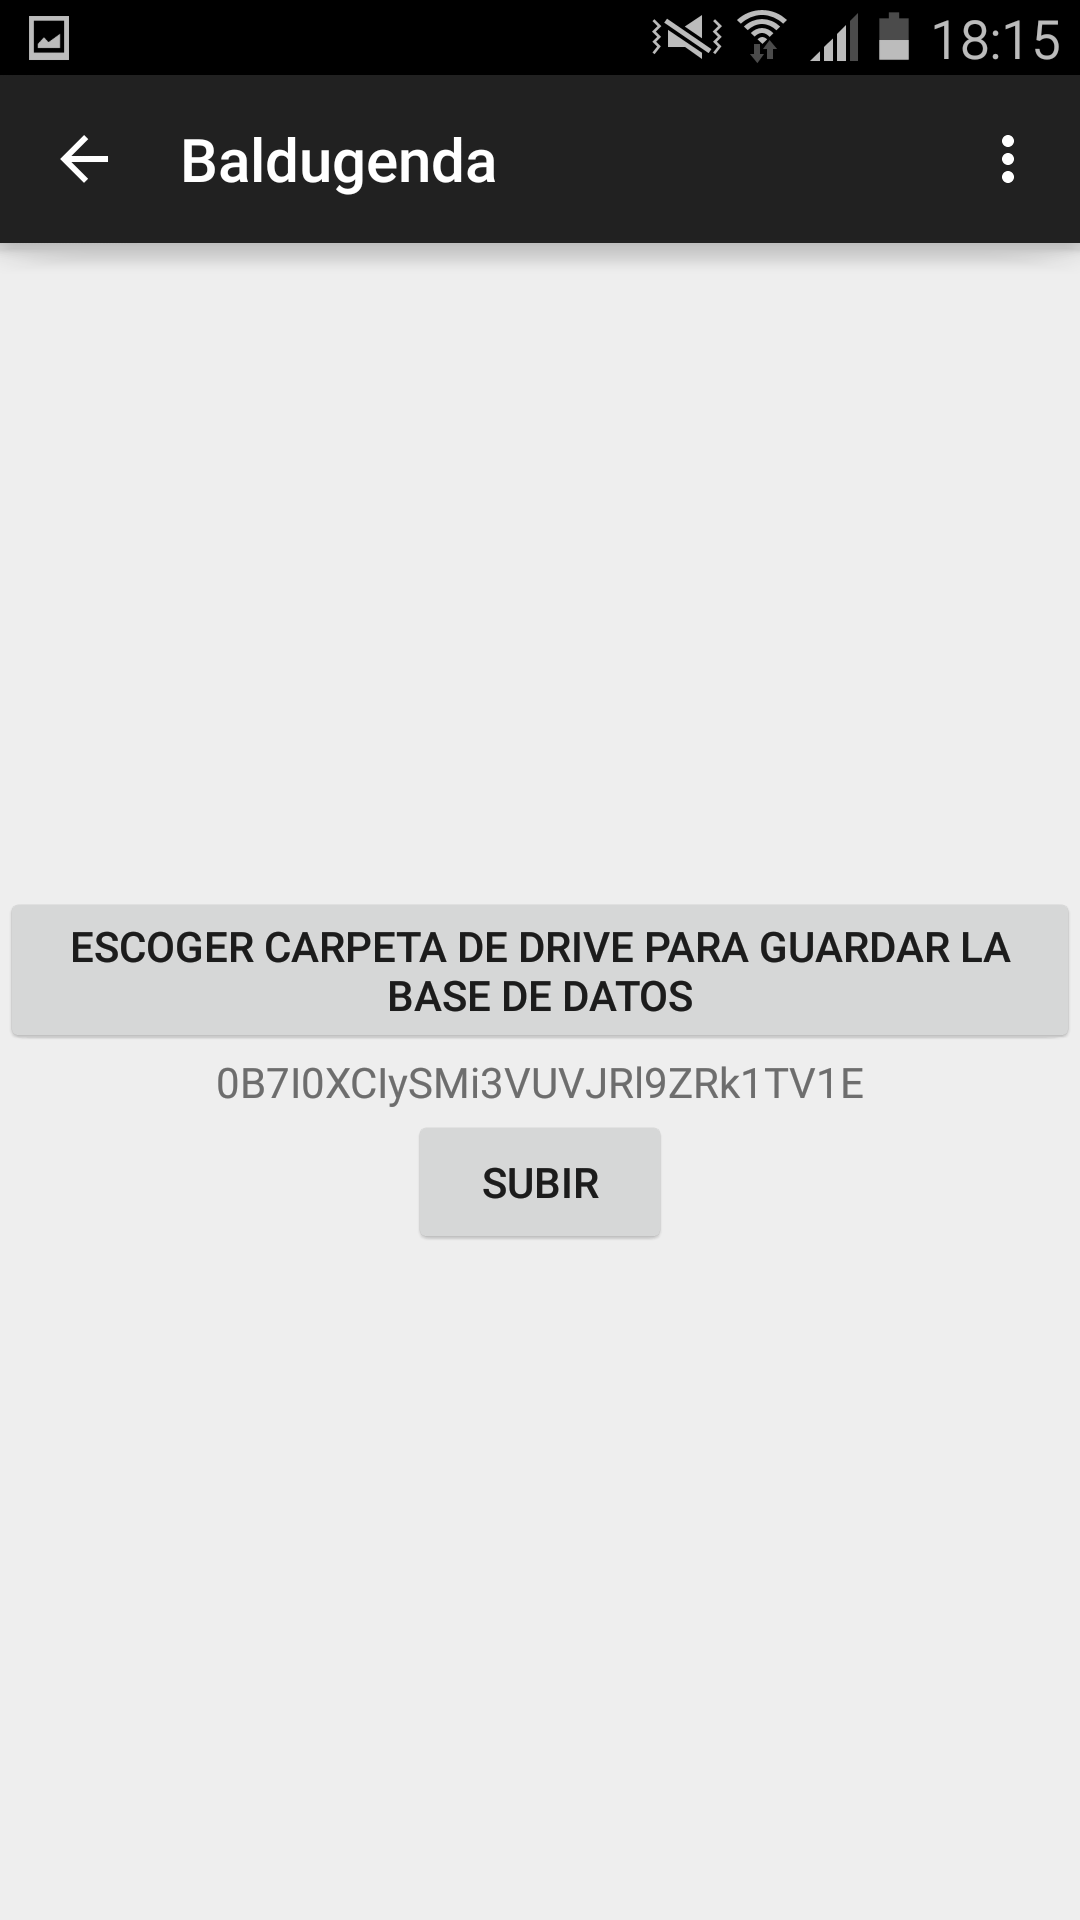
\includegraphics[width=3cm]{figs/capturas/12.png}}; 
    \node [below=of help] (importar) {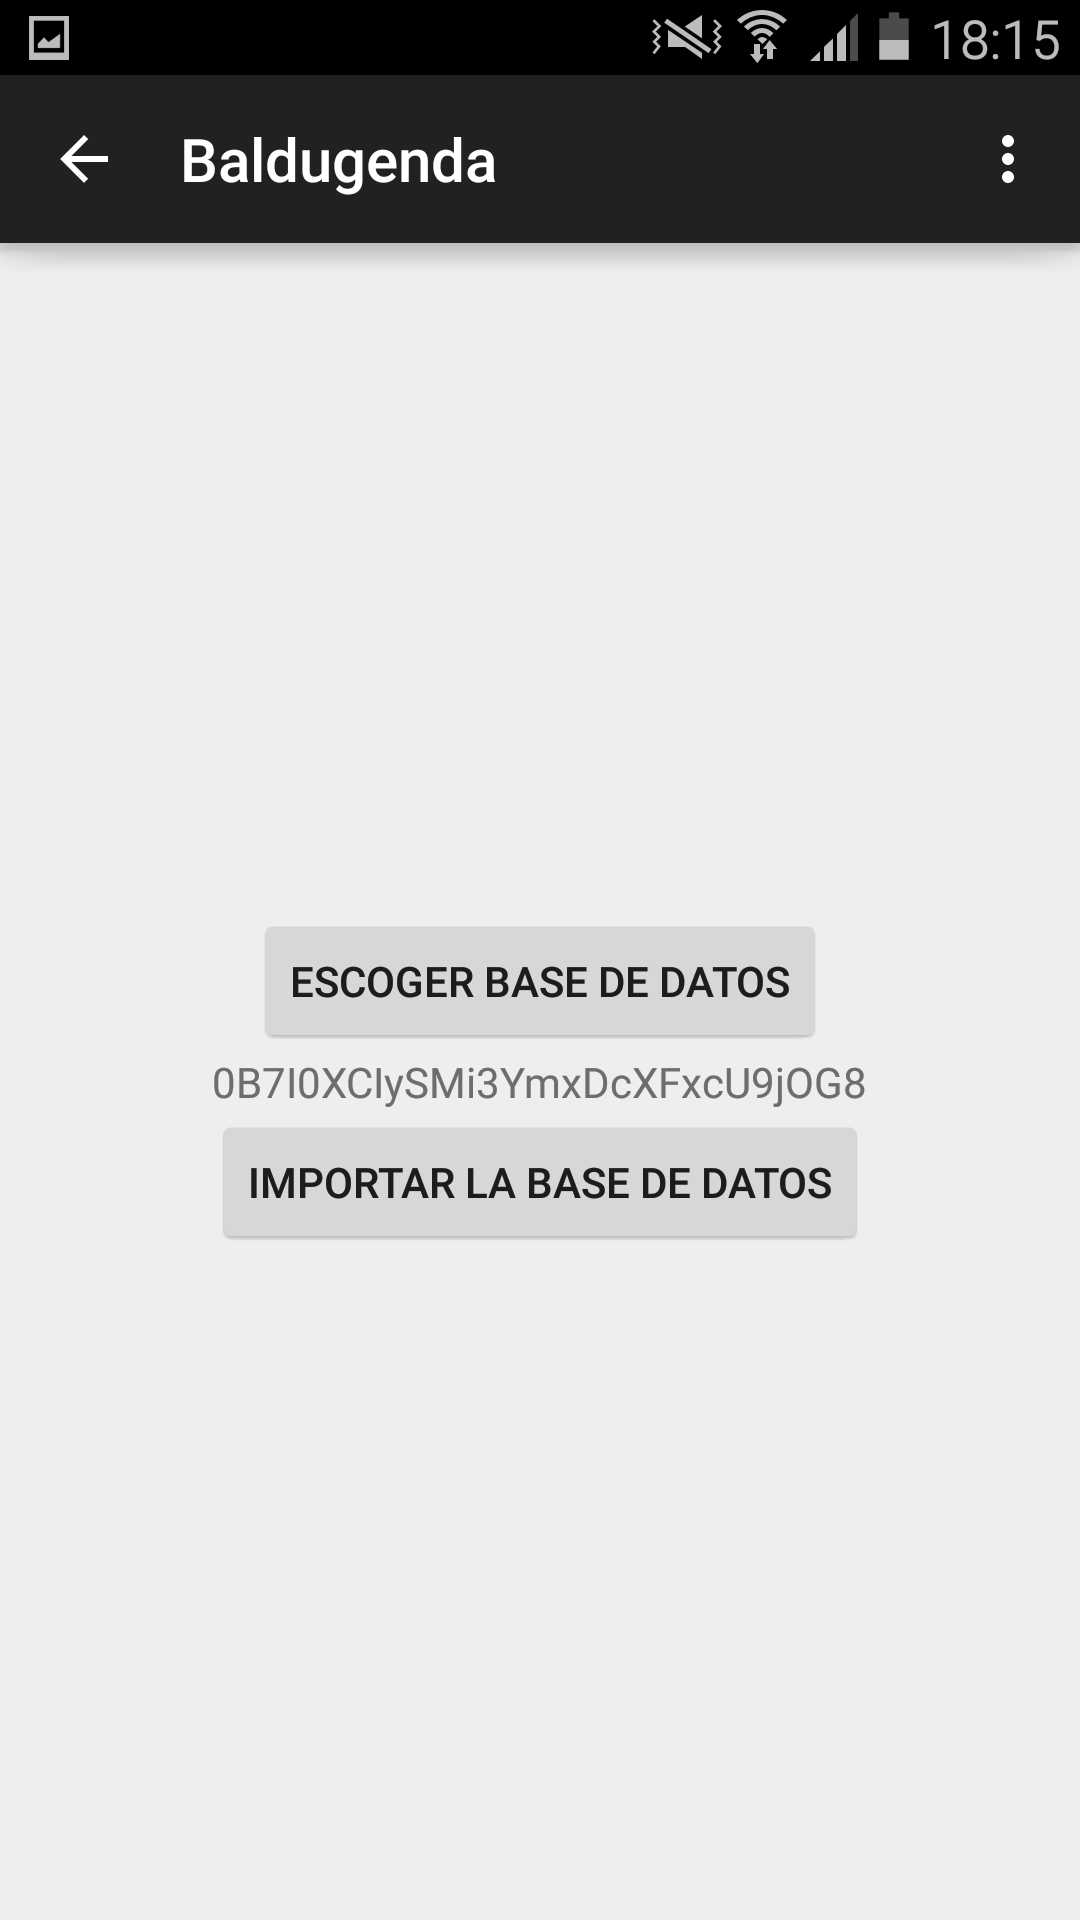
\includegraphics[width=3cm]{figs/capturas/13.png}}; 

    
    \coordinate (lista-A) at ($(main.north west) + (0.8,-1.8)$);
    \coordinate (crear-A) at ($(main.north west) + (0.8,-3.4)$);
    \coordinate (lista-E) at ($(main.north east) - (0.8,1.8)$);
    \coordinate (crear-E) at ($(main.north east) - (0.8,3.4)$);
    \coordinate (calendario) at ($(main.north west) + (0.8,-4.4)$);
    \coordinate (ayuda) at ($(main.north east) - (0.8,4.4)$);
    \coordinate (menu) at ($(main.north east) - (0.25,0.45)$);
    \draw [A] (lista-A) -- (listaAsignatura);
    \draw [A] (lista-E) -- (listaExamen);
    \draw [A] (crear-A) -- (crearAsignatura);
    \draw [A] (crear-E) -- (crearExamen);
    \draw [A] (calendario) -- (calendar);
    \draw [A] (ayuda) -- (help);
    \draw [A] (menu) -- ($(backup.north east)$);
    \draw [A] (listaAsignatura) -- (asignatura);
    \draw [A] ($(listaAsignatura.north) !0.5! (listaAsignatura.south)$) -- (modAsignatura);
    \draw [A] ($(asignatura.north) !0.5! (asignatura.south)$) -- (modAsignatura);
    \draw [A] ($(crearAsignatura.north) !0.5! (crearAsignatura.south)$) -- (asignatura);
    \draw [A] (listaExamen) -- (examen);
    \draw [A] ($(listaExamen.north) !0.5! (listaExamen.south)$) -- (modExamen);
    \draw [A] ($(examen.north) !0.5! (examen.south)$) -- (modExamen);
    \draw [A] ($(crearExamen.north) !0.5! (crearExamen.south)$) -- (examen);
    
    
  \end{tikzpicture}
  \caption{Las pantallas de la interfaz de usuario y el movimiento entre ellas}
  \label{fig:activity-relations}
\end{figure}

\subsection{Opciones adicionales de diseño}
\label{subsecc:Opciones adicionales de diseño}

Para esta aplicación se le ha dado importancia al uso de los permisos, no abusar de ellos era una de las prioridades.
En la app se piden los permisos únicos y necesarios para la conexión a Internet ademas del acceso al manejo de cuentas y calendarios en el dispositivo.
Muchas aplicaciones abusan de estos permisos, y se piden aunque en realidad no se use, porque es más fácil no tener que estar revisando los permisos que se necesitan a cada momento.
Para el desarrollo de la app se ha seguido un desarrollo por etapas y se ha optado por el uso de examinadores para probar la aplicación, y que ellos digan qué casos de uso añadirían y qué modificarían de la aplicación.
Las etapas han durado alrededor de un mes cada una de ellas y en cada nueva etapa se añadía a más personas para que probara la aplicación e hicieran comentarios.
Hay fases bien marcadas como pueden ser la fase de análisis de requisitos y la del diseño inicial. Ademas tenemos las fases de diseño detallado, en esta fase realizamos las pruebas con los usuarios y vemos las modificaciones que piden.


% Mediante los siguientes comandos, podrás compilar el conjunto de ficheros desde este mismo documento


%%% Local Variables: 
%%% mode: latex
%%% TeX-master: "../Principal"
%%% End: 


















% line in order to check if utf-8 is properly configured: áéíóúñ

\newpage
\subsection{Utilización de APIs}
\label{subsecc:Utilización de APIs}

En la aplicación de Baldugenda se ha usado 3 apis principalmente que son la de Google Calendar, Google Drive y la de Splunk Mint.
El api de Google Calendar se ha usado para el manejo de los eventos de examen dentro del calendario de Google y la creación y modificación de dichos eventos.
El api de Google Drive se ha usado para la realización del backup.
Y aunque Google nos proporciona medios para debugear la aplicación y ver qué tipos de dispositivos se la instalan se ha decidido usar el api de splunk mint para esta función ya que ofrece información específica de los errores sin que el usuario que la está usando tenga que mandar nada.

\subsection{Dispositivos}
\label{subsecc:Dispositivos}

Una de los requisitos que tenía que cumplir Baldugenda era que fuera accesible a todo el mundo que usara Android. Ya que es una labor difícil porque hay muchos dispositivos se optó por el mal menor y se fijó la versión de Android más baja posible que no diera problemas y que no quitara muchos usuarios.

La versión usada como mínimo en la aplicación fue la API 10-Gingerbread (2.3.3), según estadísticas de Google realizadas en mayo de 2015 la distribución de las versiones de Android esta así.

\begin{figure}[H] 
  \begin{center} 
    \scalebox{0.4}{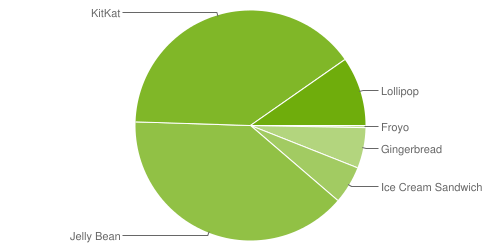
\includegraphics{figs/VersionesAndroid.png}} 
    \caption{Versiones de Android developer.android.com} 
    \label{fig:VersionesAndroid} 
  \end{center} 
\end{figure}

Aparte de la versión se tuvo que decidir para que tipo de pantallas se lanzaría la aplicación, ya que optar por todas haría que la app pesara demasiado.

Se consultó el grafico de pantallas de Google y se decidió dejar fuera la xxhdpi y a la ldpi y usar la mdpi,hdpi y xhdpi

\begin{figure}[H] 
  \begin{center} 
    \scalebox{0.4}{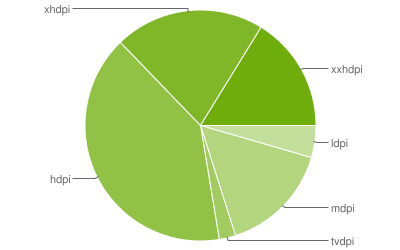
\includegraphics{figs/TiposPantalla.png}} 
    \caption{Tipos de pantalla developer.android.com} 
    \label{fig:TiposPantalla} 
  \end{center} 
\end{figure}

\subsection{Almacenamiento}
\label{subsecc:Almacenamiento}

Para el desarrollo de la aplicación se ha optado por almacenar la información en ficheros sqlite que después el programa leerá y tratara los datos. 
Durante toda la fase de implementación de la aplicación se ha ido modificando la BD hasta llegar a la versión 3 que es la que se está usando actualmente.
En cada una de las versiones se iban añadiendo campos que pedían los Baldusers, y al crear nueva versión de la BD se ha tenido que ir actualizando las BDs creadas ya en los Baldusers que ya se habían instalado la aplicación.
Estas actualizaciones eran referentes a crear columnas nuevas en las tablas o llegando a recorrer las tablas enteras para organizar los datos.
Se ha creado 3 tablas, una para las asignaturas, otra para los exámenes y la última para las notas de los exámenes.

Las tablas tienen las siguientes columnas:
\subsubsection{Asignaturas}
\label{subsubsecc:Asignaturas}


\textbf{Campo id incremental} clave primaria integer

\textbf{Nombre} campo único string, el nombre de la asignatura

\textbf{Enlaces}   un único string donde cada enlace que se presenta esta separado por “;”

\textbf{Evaluación} string que puede tener 2 valores Continua o Conjunta

\textbf{Nota} integer, será el valor máximo que se puede sacar en la asignatura

\subsubsection{Exámenes}
\label{subsubsecc:Exámenes}


\textbf{Campo id incremental} clave primaria integer

\textbf{Nombre} campo único string, el nombre del examen

\textbf{Asignatura} campo único string, el nombre de la asignatura

\textbf{Fecha} campo string, tendrá la fecha en formato DD/MM/AAAA

\textbf{Hora} campo string, tendrá la hora en formato HH:MM

\textbf{Tipo Guardado} campo string, puede tener 2 valores Ambos (si se ha podido crear el evento en Google Calendar) o Local  en caso contrario

\textbf{CalendarioId} campo string, tiene el id donde se ha generado el evento de Google Calendar

\textbf{EventoId} campo string, contiene el valor id del evento para ese examen

\textbf{CalendarioNombre} campo string, nombre del calendario donde se ha generado el evento de Google Calendar

\textbf{Descripción} campo string, descripción del examen

\subsubsection{Notas}
\label{subsubsecc:Notas}


\textbf{Campo id incremental} clave primaria integer

\textbf{Examen} campo único string, nombre del examen

\textbf{Asignatura} campo único string, nombre de la asignatura

\textbf{Nota} campo integer, nota sacada en el examen

\textbf{Nota\_Sobre} campo integer, nota máxima en el examen


Tanto en la tabla de exámenes como en la de notas se ha tenido que especificar que sea un campo único con multi valor para que no se puedan crear exámenes repetidos o duplicar notas.
A la hora de crear la base de datos se crea la BD versión 1 y la aplicación comprueba si había alguna BD en el dispositivo y que versión tiene dependiendo de eso entrara a la función de upgrade que lo que hará es realizar las actualizaciones para actualizar la BD a la versión más actual.

\subsection{Backup}
\label{subsecc:Backup}

Para esta función de Backup se ha usado el api de Google Drive, al usuario se le da la opción de exportar la base de datos a la carpeta que quiera de su Google Drive.
Para exportar primero se realiza una conexión con el servicio de Google se comprueba que tiene los permisos necesarios para realizar la creación de carpetas y ficheros y una vez Google ha mandado la respuesta, se puede acceder al Google Drive mediante una actividad que proporciona el propio api de Google Drive que muestra las carpetas del Drive y da la posibilidad de crear nuevas carpetas. 
Ya que la conexión es  asíncrona se ha tenido que separar la opción de seleccionar la carpeta donde el usuario subirá la base de datos de la opción de subir la base de datos,  si se realizaba junto al intentar subir la BD la aplicación se bloqueaba porque Google todavía no tenía la carpeta creada en su base de datos. 
A la hora de crear el fichero que se sube a Google Drive se ha realizado una transformación de un fichero a bytes.
Y después se han escrito esos bytes en el canal de entrada para el fichero que se deseaba crear.
El fichero coge el nombre de la base de datos y se le añade la fecha y la hora en la que se ha creado el fichero para que el usuario pueda escoger con facilidad ordenándolo por nombre.
Para importar la base de datos lo único que tiene que hacer el usuario es seleccionar el fichero que quiere importar y darle al botón de importar base de datos.
La lógica de negocio se encarga de coger el fichero seleccionado de Google Drive y dirigir el canal de salida del fichero escogido al fichero que se crea en la ruta de la base de datos, que en caso de que exista se borra.

\subsection{Interacción con la app}
\label{subsecc:Interacción con la app}

El manejo de Baldugenda según los Baldusers es sencillo, para acceder a la lista de asignaturas o a la lista de exámenes solo hace falta darle al icono del menú principal.
Aparte de este menú que se basa en icono con títulos que explica para que es cada icono, podemos ver las listas de asignaturas y de exámenes, cada lista tiene cosas únicas que se han colocado para probar acciones dentro de una aplicación Android.
En la lista de asignaturas se puede encontrar un menú de búsqueda para que el usuario en el caso de que tenga muchas asignaturas, escribiendo el nombre de la asignatura en la caja de texto le aparecería esa asignatura en la lista.
Aparte se ha añadido la opción de la pulsación larga en cada asignatura para poder editarla y borrarla.
En la actividad de exámenes se puede ver que la lista no es igual a la lista de asignaturas, se ha usado la clase ExpandableList para crear cajones donde ira la asignatura y los exámenes de esa asignatura, junto con el número de exámenes que hay dentro de la asignatura.
Se ha modificado el botón de atrás dentro de la actividad lista exámenes para que muestre un menú de navegación lateral para poder ir a cualquiera de las actividades mostradas. A los Baldusers les pareció bien el menú pero ninguno vio necesario ponerlo en cada actividad.




% Mediante los siguientes comandos, podrás compilar el conjunto de ficheros desde este mismo documento


%%% Local Variables: 
%%% mode: latex
%%% TeX-master: "../Principal"
%%% End: 


















% line in order to check if utf-8 is properly configured: áéíóúñ